%! Mode:: "TeX:UTF-8"
%! TEX program = xelatex
\PassOptionsToPackage{quiet}{xeCJK}
\documentclass[withoutpreface,bwprint]{cumcmthesis}
\usepackage{etoolbox}
\BeforeBeginEnvironment{tabular}{\zihao{-5}}
\usepackage[numbers,sort&compress]{natbib}  % 文献管理宏包
\usepackage[framemethod=TikZ]{mdframed}  % 框架宏包
\usepackage{url}  % 网页链接宏包
\usepackage{subcaption}  % 子图宏包
\usepackage{float}  % 浮动体宏包

\newcolumntype{C}{>{\centering\arraybackslash}X}
\newcolumntype{R}{>{\raggedleft\arraybackslash}X}
\newcolumntype{L}{>{\raggedright\arraybackslash}X}

\title{全国大学生数学建模竞赛论文模板}  % 论文标题
\tihao{}  % 题号
\baominghao{}  % 报名号
\schoolname{}  % 学校
\membera{}  % 队员a
\memberb{}  % 队员b
\memberc{}  % 队员c
\supervisor{}  % 指导老师
\yearinput{}
\monthinput{}
\dayinput{}

%%%%%%%%%%%%%%%%%%%%%%%%%%%%%%%%%%%%%%%%%%%%%%%%%%%%%%%%%%%%%
%% 正文
\begin{document}

\maketitle
\begin{abstract}
摘要

\textbf{对于问题一,}

\textbf{对于问题二,}

\textbf{对于问题三,}

\textbf{对于问题四,}

最后,



\keywords{关键词\quad  关键词\quad  关键词\quad  关键词 \quad 关键词}
\end{abstract}
%%%%%%%%%%%%%%%%%%%%%%%%%%%%%%%%%%%%%%%%%%%%%%%%%%%%%%%%%%%%% 

% \tableofcontents  % 目录
% \newpage

%%%%%%%%%%%%%%%%%%%%%%%%%%%%%%%%%%%%%%%%%%%%%%%%%%%%%%%%%%%%%  
\section{问题重述}
\subsection{问题背景}
丝绸之路作为古代中西方文化交流的核心通道,玻璃是早期贸易往来的重要物证。
早期西亚和埃及的玻璃多以珠形饰品传入我国,我国古代吸收其技术后,
利用本土原料制作玻璃,虽外观与外来品相似,但因助熔剂差异(如铅矿石、草木灰等),
化学成分截然不同,形成了铅钡玻璃(我国自创,以楚文化为代表)、
高钾玻璃(流行于岭南及东南亚、印度等区域)等本土特色品种。
古代玻璃因埋藏环境易风化,风化过程中元素交换导致成分比例改变,
影响类别判断,而部分风化文物表面仍保留未风化区域,为成分研究提供了特殊样本,
对于研究古代中国社会和玻璃工艺具有很高的价值。

%%%%%%%%%%%%%%%%%%%%%%%%%%%%%%%%%%%%%%%%%%%%%%%%%%%%%%%%%%%%% 

\subsection{问题要求}

\textbf{问题1}  
分析玻璃文物的表面风化状态与其类型(高钾玻璃 / 铅钡玻璃)、
纹饰、颜色之间的关联;结合玻璃类型,
总结文物表面有无风化时化学成分含量的统计规律;
并基于风化点的检测数据,预测其风化前的化学成分含量。

\textbf{问题2}  
依据附件数据,提炼高钾玻璃与铅钡玻璃的分类规律;
针对这两类玻璃,分别选取合适的化学成分进行亚类划分,
明确具体的划分方法及结果,并分析该分类结果的合理性与敏感性。

\textbf{问题3} 
对附件表单 3 中未知类别的玻璃文物,通过分析其化学成分鉴别其所属类型
(高钾玻璃或铅钡玻璃),并对该分类结果的敏感性进行分析。

\textbf{问题4}  
针对高钾玻璃和铅钡玻璃这两类不同的文物样品,
分别分析其内部化学成分之间的关联关系,
并比较两类玻璃在化学成分关联关系上的差异性。
%%%%%%%%%%%%%%%%%%%%%%%%%%%%%%%%%%%%%%%%%%%%%%%%%%%%%%%%%%%%% 

\section{问题分析}
\subsection{问题一分析}
对于问题一,

\subsection{问题二分析}	
对于问题二,

\subsection{问题三分析}
对于问题三,

\subsection{问题四分析}
对于问题四,

%%%%%%%%%%%%%%%%%%%%%%%%%%%%%%%%%%%%%%%%%%%%%%%%%%%%%%%%%%%%% 

\section{模型假设}

为简化问题,本文做出以下假设:

\begin{itemize}[itemindent=2em]
\item 假设1
\item 假设2
\item 假设3
\end{itemize}

%%%%%%%%%%%%%%%%%%%%%%%%%%%%%%%%%%%%%%%%%%%%%%%%%%%%%%%%%%%%% 

\section{符号说明}
\begin{table}[H]
\centering
\begin{tabularx}{\textwidth}{CLC}
\toprule
符号    & 说明    & 单位 \\
\midrule
$m     $& 质量 & $kg$ \\
$V     $& 体积 & $m^3$ \\
\bottomrule
\end{tabularx}
\label{tab:符号说明}
\end{table}


%%%%%%%%%%%%%%%%%%%%%%%%%%%%%%%%%%%%%%%%%%%%%%%%%%%%%%%%%%%%% 

\section{问题一的模型的建立和求解}
\subsection{玻璃类型、颜色、纹饰与风化的关系}
首先我们对表单2中各文物采样点的化学成分进行累加,其中样本编号为15、17的文物
化学成分总和分别为79.47\%、71.89\%,不满足题目对成分比例累加和介于 
85\%~105\%之间的要求,因此我们将其剔除。

为了分析表面风化与玻璃类型、纹饰、颜色之间的关系,我们分别统计
(表面风化,玻璃类型)(表面风化,纹饰)(表面风化,颜色)这三个二元组
的列联表数据,并进行了可视化。

% 表1:表面风化与颜色的列联表(单独一行)
\begin{table}[htbp]
    \centering
    \caption{表面风化与颜色的列联表}
    \begin{tabular}{lcccccccc}
        \toprule
        \multirow{2}{*}{表面风化} & \multicolumn{8}{c}{颜色} \\
        \cmidrule(lr){2-9}
        & 浅绿 & 浅蓝 & 深绿 & 深蓝 & 紫 & 绿 & 蓝绿 & 黑 \\
        \midrule
        无风化 & 2 & 6 & 3 & 2 & 2 & 1 & 6 & 0 \\
        风化 & 1 & 12 & 4 & 0 & 2 & 0 & 9 & 2 \\
        \bottomrule
    \end{tabular}
\end{table}

% 表2和表3并排显示(同一行)
\begin{table}[htbp]
    \centering
    % 表2:表面风化与纹饰
    \caption{表面风化与纹饰、玻璃类型的列联表} % 总标题(可选)
    \begin{subtable}[t]{0.45\textwidth}
        \centering
        \caption{表面风化与纹饰的列联表}
        \begin{tabular}{lccc}
            \toprule
            \multirow{2}{*}{表面风化} & \multicolumn{3}{c}{纹饰} \\
            \cmidrule(lr){2-4}
            & A & B & C \\
            \midrule
            无风化 & 11 & 0 & 11 \\
            风化 & 11 & 6 & 17 \\
            \bottomrule
        \end{tabular}
    \end{subtable}
    \hspace{-15mm}% 两表之间的水平间距
    % 表3:表面风化与玻璃类型
    \begin{subtable}[t]{0.45\textwidth}
        \centering
        \caption{表面风化与玻璃类型的列联表}
        \begin{tabular}{lcc}
            \toprule
            \multirow{2}{*}{表面风化} & \multicolumn{2}{c}{类型} \\
            \cmidrule(lr){2-3}
            & 铅钡 & 高钾 \\
            \midrule
            无风化 & 12 & 10 \\
            风化 & 28 & 6 \\
            \bottomrule
        \end{tabular}
    \end{subtable}
\end{table}

\begin{figure}[H]
\centering
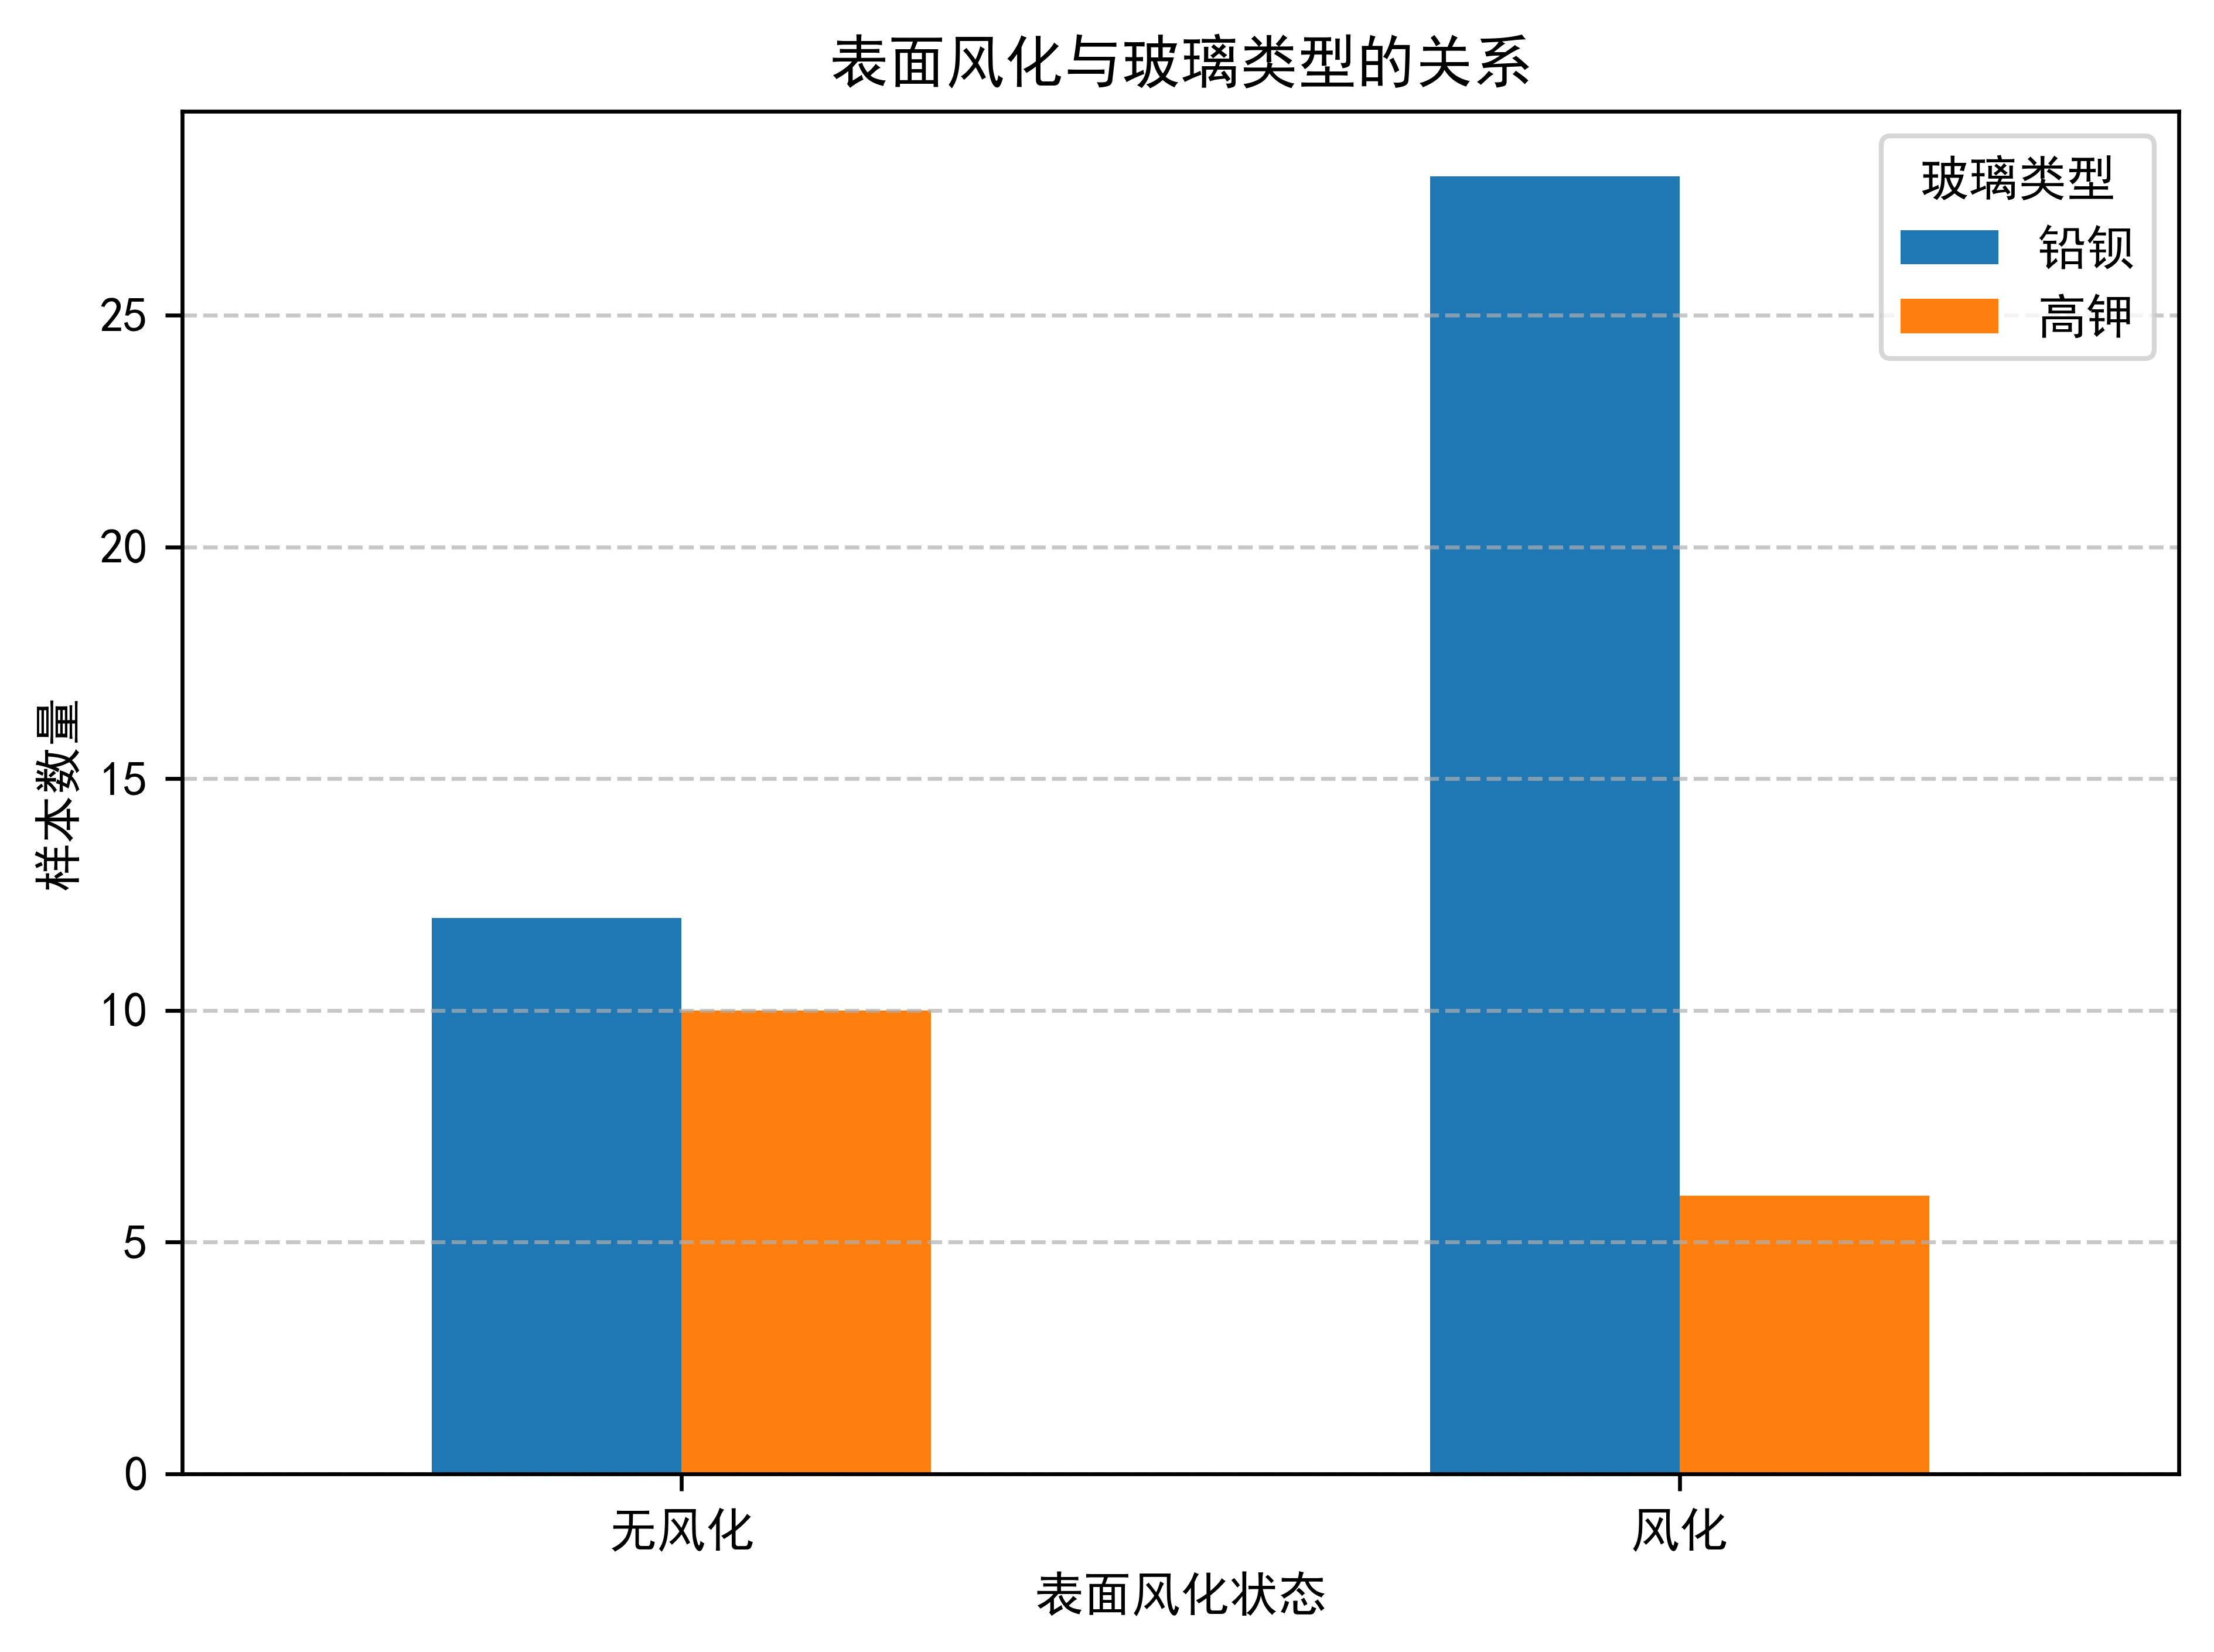
\includegraphics[width=0.6\textwidth]{figures/1.1/1-1.png}
\caption{表面风化与玻璃类型}
\label{fig:表面风化与玻璃类型}
\end{figure}

\begin{figure}[H]
\centering
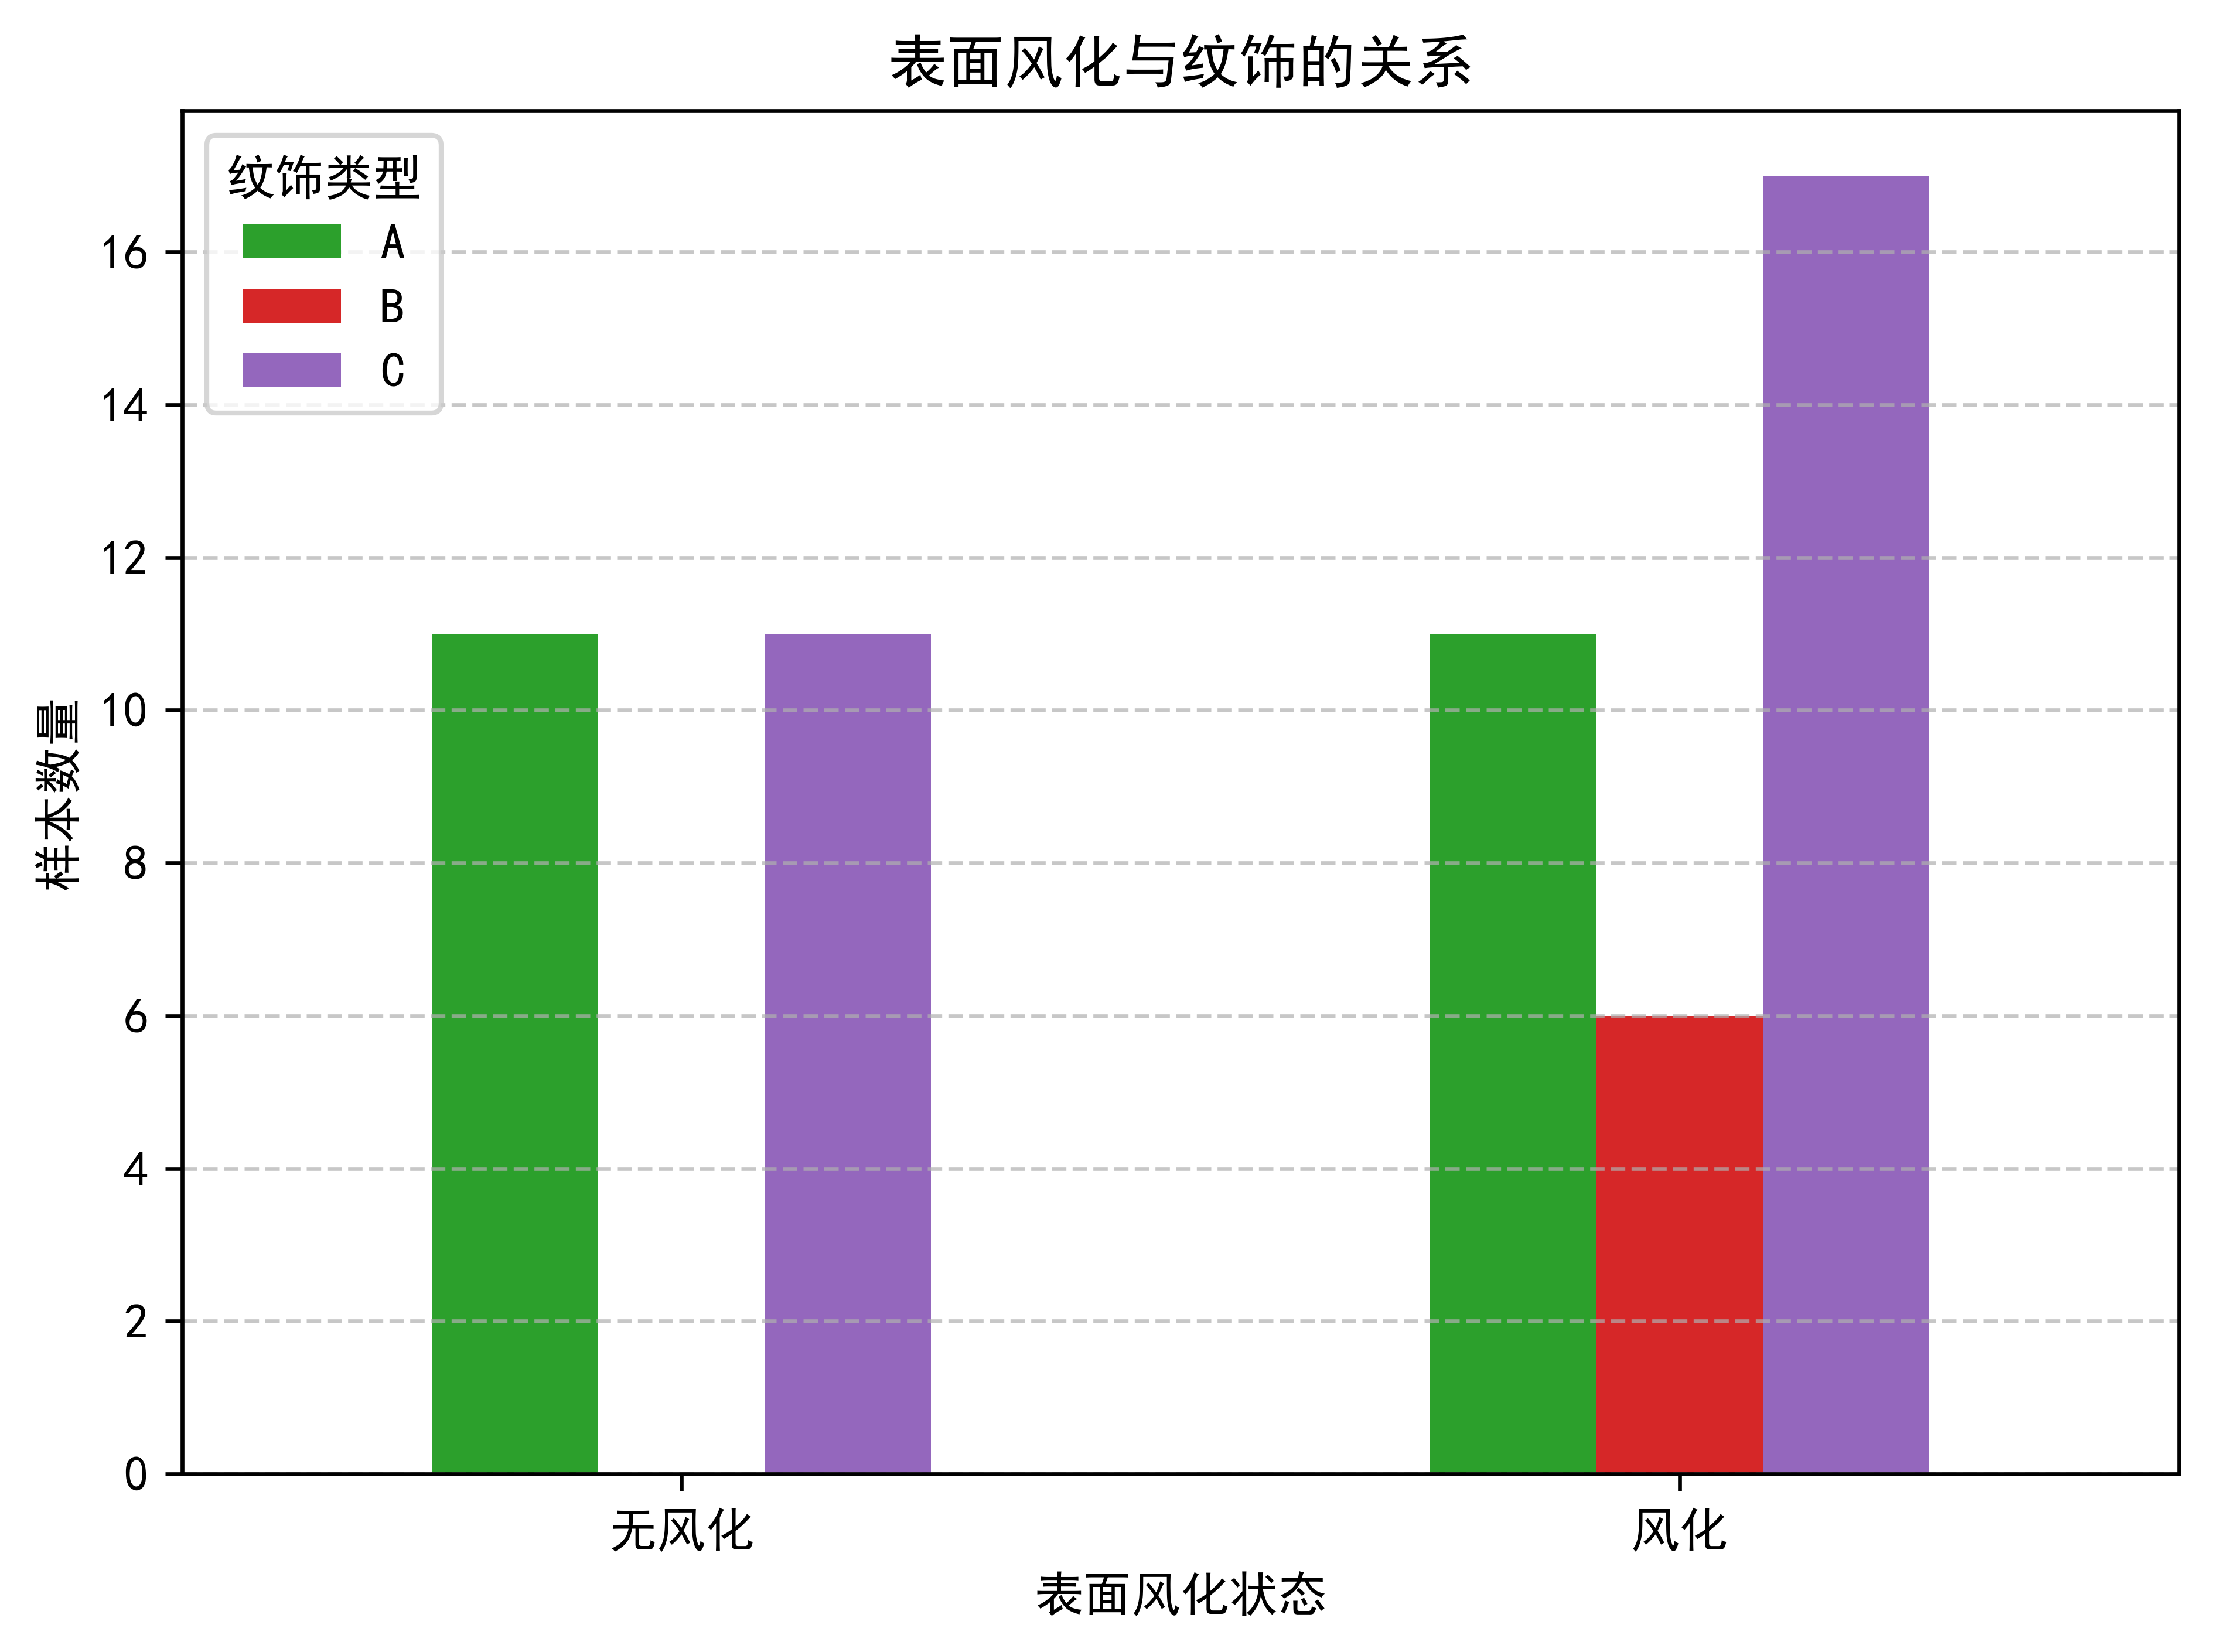
\includegraphics[width=0.6\textwidth]{figures/1.1/1-2.png}
\caption{表面风化与纹饰}
\label{fig:表面风化与纹饰}
\end{figure}

\begin{figure}[H]
\centering
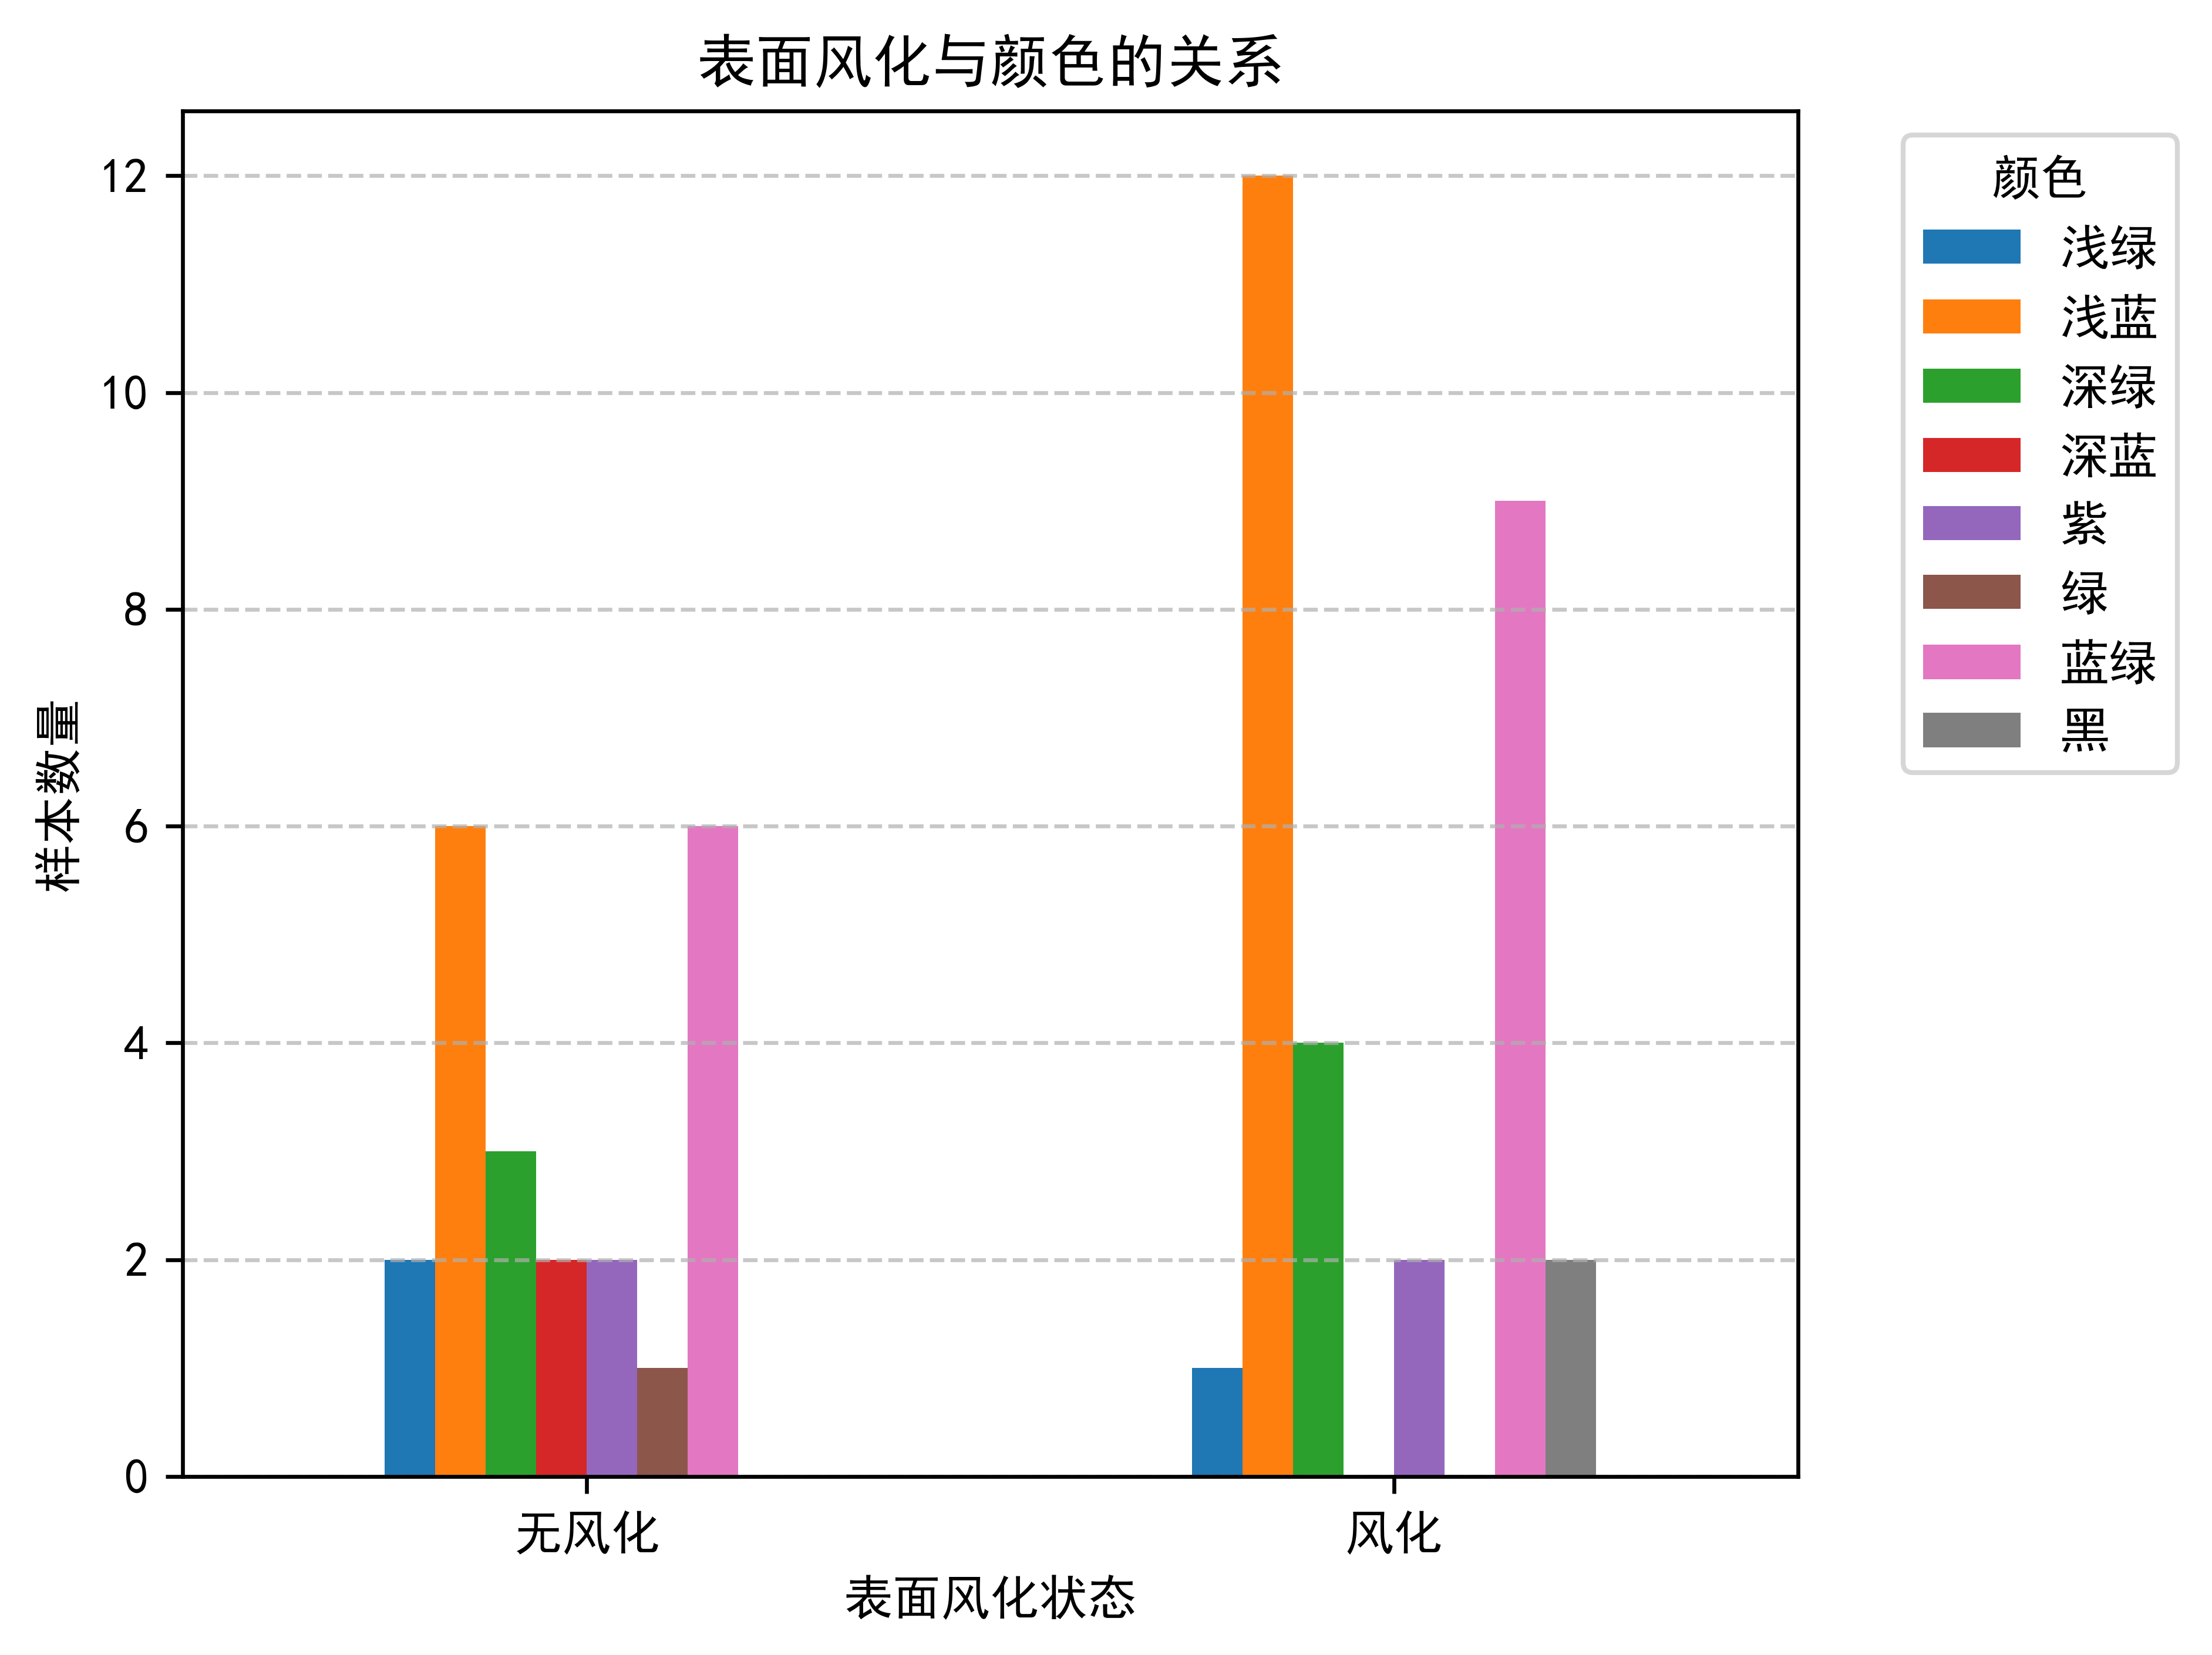
\includegraphics[width=0.6\textwidth]{figures/1.1/1-3.png}
\caption{表面风化与颜色}
\label{fig:表面风化与颜色}
\end{figure}

为了量化表面风化与玻璃类型、纹饰、颜色之间的关系,我们引入了卡方检验。
卡方检验用于检验两个分类变量是否独立,通过比较观测值与期望值的差异,
用 $\chi^2$ 统计量判断关联是否显著,适用于计数数据。

%引用公式\cref{eq:公式1}。

\begin{equation}
\label{eq:公式1}
\chi^2 = \sum \frac{(O - E)^2}{E}
\end{equation}

其中:
 $\chi^2$:卡方统计量;
 $O$:实际观测频数;
 $E$:理论期望频数;
 $\sum$:对所有单元格求和。

分别带入(表面风化,玻璃类型)(表面风化,纹饰)(表面风化,颜色)的
列联表数据可以求出$\chi^2$值和$p$值,我们这里取$p<0.005$。从下面的表格中我们可以看出,
是否风化与玻璃类型之间存在显著关系,而风化与纹饰、颜色之间则不存在显著关系。

\begin{table}[htbp]
    \centering
    \caption{卡方检验结果}
    \begin{tabular}{lcccc}
        \toprule
        关系 & $\chi^2$ & $df$ & $p$值 &  是否显著 \\
        \midrule
        风化 $\times$ 颜色 & 7.0114 & 7 & $p \approx 0.426$ & 否 \\
        风化 $\times$ 纹饰 & 4.9412 & 2 & $p \approx 0.085$ & 否 \\
        风化 $\times$ 类型 & 5.0610 & 1 & $p \approx 0.024$ & 是 \\
        \bottomrule
    \end{tabular}
\end{table}

\subsection{玻璃是否风化化学成分含量的统计规律}

以文物采样点为单位,以玻璃类型、是否风化为分组依据,将数据分为四个组别:

\begin{enumerate}
    \item 无风化铅钡玻璃
    \item 无风化高钾玻璃
    \item 风化铅钡玻璃
    \item 风化高钾玻璃
\end{enumerate}

我们对预处理后的数据进行统计,计算出了每种组别的化学成分含量的均值、
极差、方差、有效样本数。同时,为了更直观的看出化学成分的变化,我们将
同一化学成分的风化前后含量做成了柱状图,以下进行部分展示。

% 铅钡无风化表格
\begin{table}[htbp]
    \centering
    \caption{铅钡无风化样本化学成分统计数据}
    \begin{tabular}{lccccc}
        \hline
        化学成分 & 均值 & 极差 & 方差 & 有效样本数 \\
        \hline
        二氧化硅(SiO₂) & 53.4438 & 43.5700 & 212.7885 & 13 \\
        氧化钠(Na₂O) & 3.3433 & 2.0000 & 1.3008 & 3 \\
        氧化钾(K₂O) & 0.4356 & 1.4600 & 0.2193 & 9 \\
        氧化钙(CaO) & 1.3909 & 4.1100 & 2.2167 & 11 \\
        氧化镁(MgO) & 1.4812 & 4.9400 & 2.6958 & 8 \\
        氧化铝(Al₂O₃) & 2.8915 & 3.5600 & 1.6320 & 13 \\
        氧化铁(Fe₂O₃) & 2.1240 & 4.4200 & 2.8855 & 5 \\
        氧化铜(CuO) & 1.8400 & 8.3500 & 6.8727 & 11 \\
        氧化铅(PbO) & 23.5938 & 29.9200 & 82.7080 & 13 \\
        氧化钡(BaO) & 24.4662 & 23.2300 & 62.8734 & 13 \\
        五氧化二磷(P₂O₅) & 1.0682 & 5.6500 & 2.7670 & 11 \\
        氧化锶(SrO) & 0.4825 & 0.6800 & 0.0664 & 8 \\
        氧化锡(SnO₂) & 0.4000 & 0.0000 & nan & 1 \\
        二氧化硫(SO₂) & 2.0500 & 3.2200 & 5.1842 & 2 \\
        \hline
    \end{tabular}
\end{table}

% 铅钡风化表格
\begin{table}[htbp]
    \centering
    \caption{铅钡风化样本化学成分统计数据}
    \begin{tabular}{lccccc}
        \hline
        化学成分 & 均值 & 极差 & 方差 & 有效样本数 \\
        \hline
        二氧化硅(SiO₂) & 33.6147 & 64.3600 & 296.5795 & 36 \\
        氧化钠(Na₂O) & 3.1173 & 7.1200 & 5.4794 & 11 \\
        氧化钾(K₂O) & 0.3937 & 1.3000 & 0.1208 & 16 \\
        氧化钙(CaO) & 2.4835 & 6.0300 & 2.4015 & 34 \\
        氧化镁(MgO) & 1.0970 & 2.2600 & 0.2306 & 23 \\
        氧化铝(Al₂O₃) & 3.8383 & 13.8900 & 11.6460 & 36 \\
        氧化铁(Fe₂O₃) & 0.9529 & 2.5500 & 0.4407 & 21 \\
        氧化铜(CuO) & 2.1135 & 10.3800 & 6.3094 & 34 \\
        氧化铅(PbO) & 36.8719 & 57.9000 & 229.9385 & 36 \\
        氧化钡(BaO) & 34.5803 & 64.8600 & 297.0158 & 35 \\
        五氧化二磷(P₂O₅) & 4.9863 & 14.0600 & 16.5052 & 30 \\
        氧化锶(SrO) & 0.4122 & 1.0000 & 0.0484 & 32 \\
        氧化锡(SnO₂) & 0.7700 & 1.0800 & 0.5832 & 2 \\
        二氧化硫(SO₂) & 7.1980 & 15.4800 & 57.9916 & 5 \\
        \hline
    \end{tabular}
\end{table}

% 高钾无风化表格
\begin{table}[htbp]
    \centering
    \caption{高钾无风化样本化学成分统计数据}
    \begin{tabular}{lccccc}
        \hline
        化学成分 & 均值 & 极差 & 方差 & 有效样本数 \\
        \hline
        二氧化硅(SiO₂) & 67.9842 & 28.0400 & 76.6518 & 12 \\
        氧化钠(Na₂O) & 2.7800 & 1.2800 & 0.4144 & 3 \\
        氧化钾(K₂O) & 9.7233 & 9.8100 & 9.2269 & 12 \\
        氧化钙(CaO) & 6.0500 & 7.4800 & 6.6337 & 10 \\
        氧化镁(MgO) & 1.3033 & 1.4600 & 0.2784 & 9 \\
        氧化铝(Al₂O₃) & 6.6200 & 8.1000 & 6.2076 & 12 \\
        氧化铁(Fe₂O₃) & 2.3180 & 5.6200 & 2.4002 & 10 \\
        氧化铜(CuO) & 2.6755 & 4.6200 & 2.3750 & 11 \\
        氧化铅(PbO) & 0.7057 & 1.5100 & 0.3939 & 7 \\
        氧化钡(BaO) & 1.4360 & 2.8600 & 1.1488 & 5 \\
        五氧化二磷(P₂O₅) & 1.5300 & 4.3400 & 2.0473 & 11 \\
        氧化锶(SrO) & 0.0833 & 0.0800 & 0.0010 & 6 \\
        氧化锡(SnO₂) & 2.3600 & 0.0000 & nan & 1 \\
        二氧化硫(SO₂) & 0.4067 & 0.1100 & 0.0032 & 3 \\
        \hline
    \end{tabular}
\end{table}

% 高钾风化表格
\begin{table}[htbp]
    \centering
    \caption{高钾风化样本化学成分统计数据}
    \begin{tabular}{lccccc}
        \hline
        化学成分 & 均值 & 极差 & 方差 & 有效样本数 \\
        \hline
        二氧化硅(SiO₂) & 93.9633 & 4.4200 & 3.0054 & 6 \\
        氧化钾(K₂O) & 0.7040 & 0.7500 & 0.0879 & 5 \\
        氧化钙(CaO) & 0.8700 & 1.4500 & 0.2379 & 6 \\
        氧化镁(MgO) & 0.5900 & 0.1000 & 0.0050 & 2 \\
        氧化铝(Al₂O₃) & 1.9300 & 2.6900 & 0.9302 & 6 \\
        氧化铁(Fe₂O₃) & 0.2650 & 0.1800 & 0.0048 & 6 \\
        氧化铜(CuO) & 1.5617 & 2.6900 & 0.8739 & 6 \\
        五氧化二磷(P₂O₅) & 0.3360 & 0.4600 & 0.0316 & 5 \\
        \hline
    \end{tabular}
\end{table}

\begin{figure}[H]
\centering
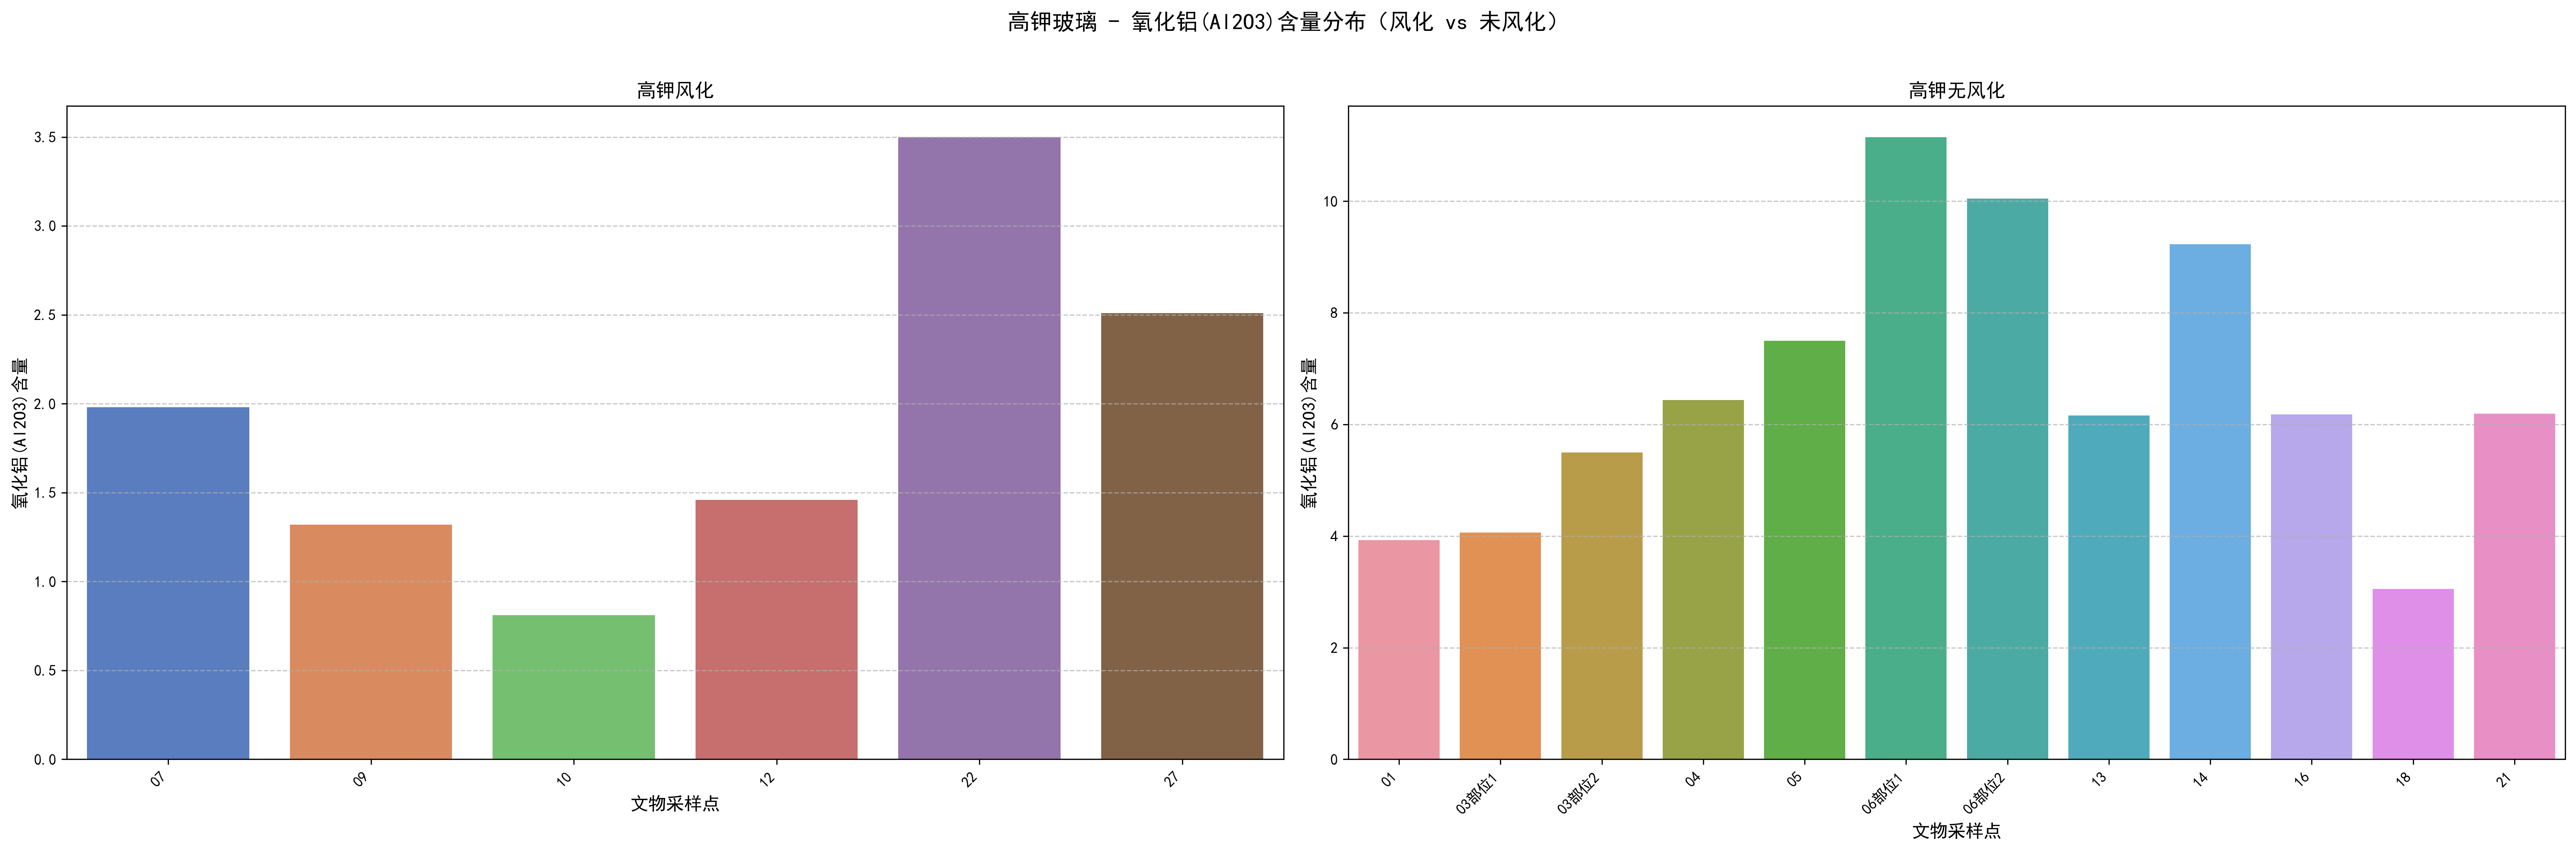
\includegraphics[width=0.9\textwidth]{figures/1.2/高钾玻璃 - 氧化铝(Al2O3)含量分布(风化 vs 未风化).png}
\caption{高钾玻璃 - 氧化铝(Al$_2$O$_3$)风化前后含量分布}
\label{fig:高钾玻璃 - 氧化铝(Al$_2$O$_3$)风化前后含量分布}
\end{figure}

\begin{figure}[H]
\centering
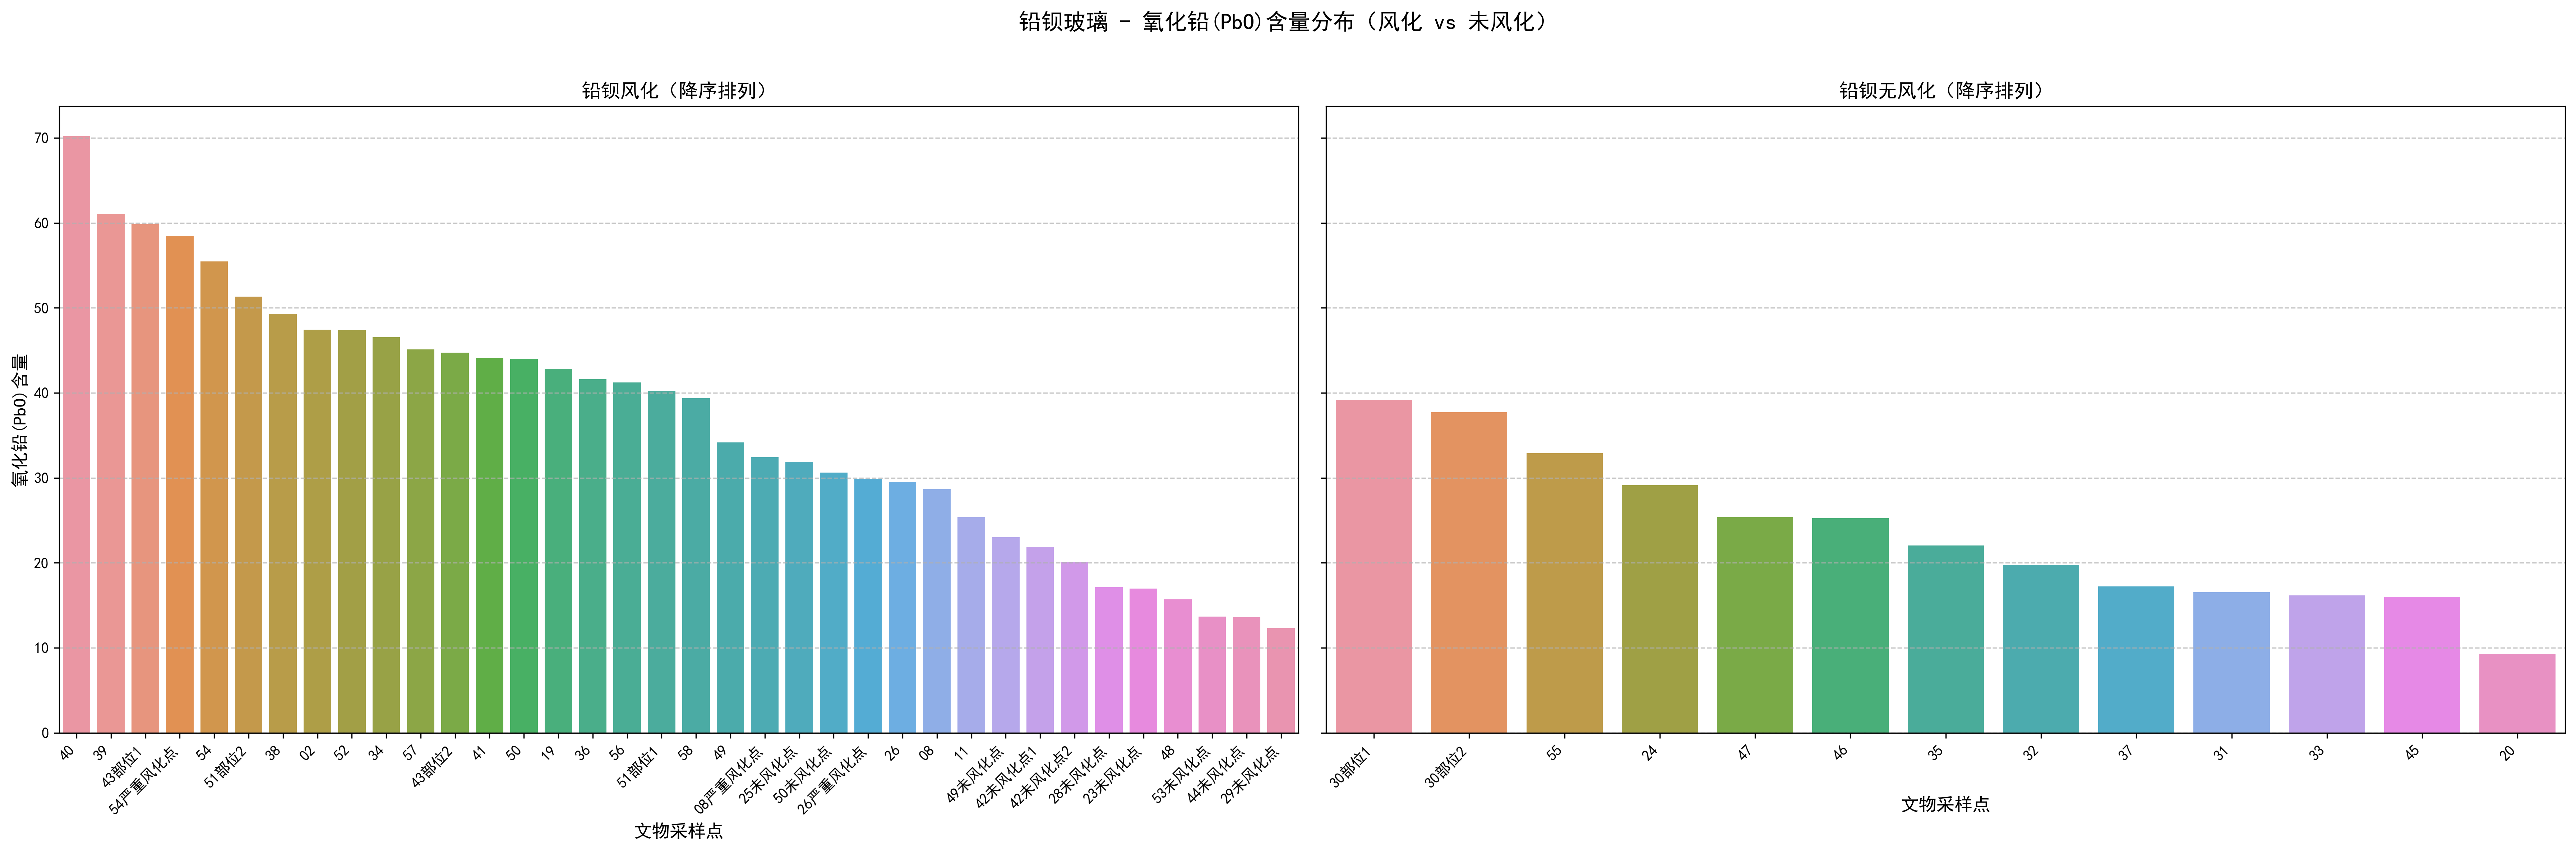
\includegraphics[width=0.9\textwidth]{figures/1.2/铅钡玻璃 - 氧化铅(PbO)含量分布(风化 vs 未风化).png}
\caption{铅钡玻璃 - 氧化铅(PbO)风化前后含量分布}
\label{fig:铅钡玻璃 - 氧化铅(PbO)风化前后含量分布}
\end{figure}

\begin{figure}[H]
\centering
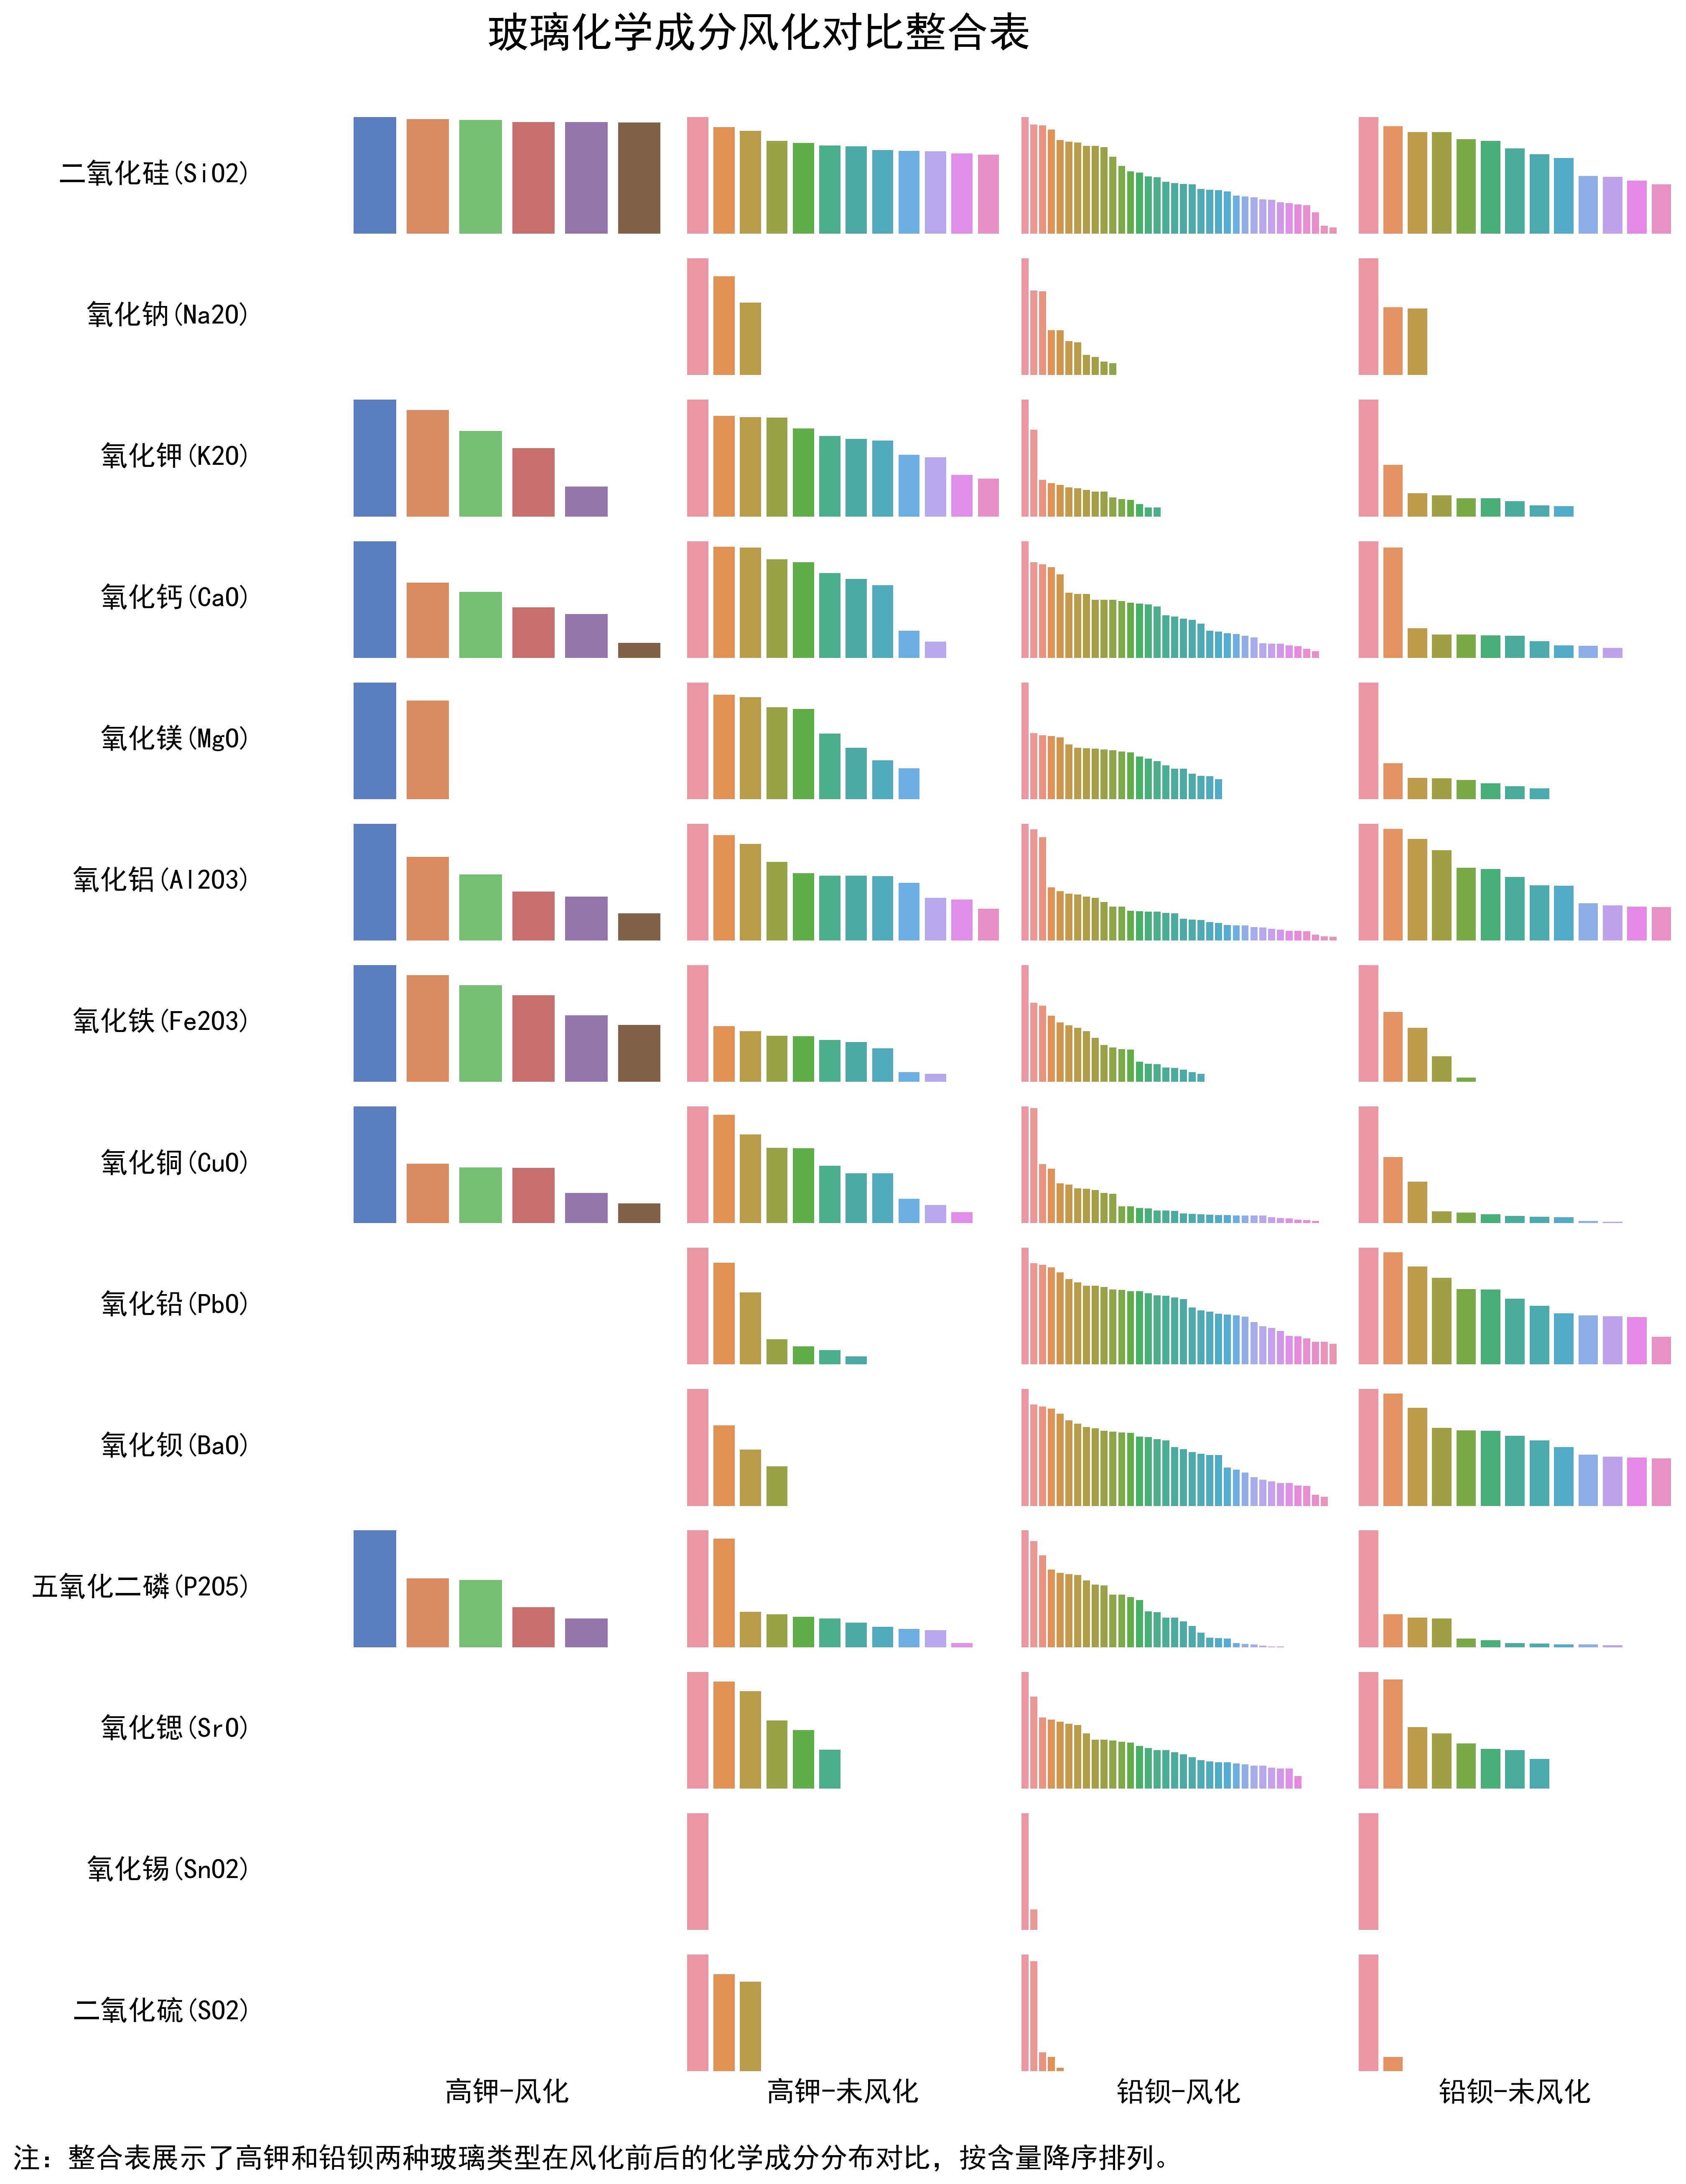
\includegraphics[width=0.9\textwidth]{figures/1.2/玻璃化学成分风化对比整合表(14x4)V3.png}
\caption{高钾-铅钡玻璃风化前后各化学含量对比}
\label{fig:高钾-铅钡玻璃风化前后各化学含量对比}
\end{figure}

通过这些图表,可以直观地观察到:

\begin{itemize}
    \item 铅钡玻璃在风化后,SiO$_2$含量略微增加,而 SrO、Fe$_2$O$_3$、CuO、Na$_2$O、MgO、CaO、K$_2$O、Al$_2$O$_3$、PbO、BaO、P$_2$O$_5$ 和 SO$_2$ 含量均有不同程度的下降;
    \item 高钾玻璃在风化后,SiO$_2$含量显著降低,而 SrO、Fe$_2$O$_3$、CuO、Na$_2$O、MgO、CaO、K$_2$O、Al$_2$O$_3$、PbO、BaO、P$_2$O$_5$ 和 SO$_2$ 含量明显增加,SnO$_2$含量基本不变;
    \item 风化过程对不同类型玻璃的化学成分影响存在明显差异。
\end{itemize}

\subsection{风化前的化学成分含量的预测}

\subsubsection{数据分析}

通过阅读数据,我们发现,除了编号为49、50的样本具有成对的(风化前,风化后)的化学成分数据,
其他的样本都是基于风化前后两群体的横截面数据,可以抽象为(风化前,NULL)或(NULL,风化后)
的形式。同时,考虑到需要预测的是化学成分,是总和为1的成分数据,各成分之间彼此依赖,
不适宜使用一般的回归模型。

因此,我们基于成分数据分析CoDA模型,参考文献\cite{司守奎2011数学建模算法与应用},
在模型中添加先验正则项,最终建立风化前化学含量预测模型。

\subsubsection{模型记号与数据映射}

\begin{itemize}
\item 模型记号
\begin{itemize}
    \item $\mathbf{a}_i$ \quad (原始成分百分比)  
    \item $\mathbf{p}_i$ \quad (闭合后,和为 1 的比例)  
    \item $\mathbf{z}_i$ \quad (clr 后的向量)  
    \item $\bar{\mathbf{z}}_\text{w},\, \bar{\mathbf{z}}_\text{u}$ \quad  
    \item $\boldsymbol{\delta}_0$ \quad (按玻璃类型用文献导向值初始化)  
    \item $\mathbf{w}$ \quad (按成分设置权重)  
    \item $\lambda$ \quad (正则强度) 
    \item $n$ \quad (样本数)
\end{itemize}

\item 令成分列为:
\[
    \mathcal{P} = \{\mathrm{SiO}_2, \mathrm{Na}_2\mathrm{O}, \mathrm{K}_2\mathrm{O}, \ldots, \mathrm{SO}_2, \text{unknown}\}
\]
共 $D = 15$ 个成分

\item 将每行按百分比除以 100 进行闭合,得到组成比例矩阵 $\mathbf{p} \in \mathbb{R}^{n \times D}$。
    \begin{itemize}
        \item 样本 $i$ 的成分向量为 $\mathbf{a}_i$,闭合后
        \[
        \mathbf{p}_i = \mathcal{C}(\mathbf{a}_i) = \frac{\mathbf{a}_i}{\sum_{j=1}^D a_{ij}}, \quad \sum_{j=1}^D p_{ij} = 1.
        \]
    \end{itemize}

\item 为避免 $\log(0)$,在闭合前/或闭合后对零值做微小替换(伪计数)$\varepsilon$。

\item CLR 变换(把单纯形映到实向量空间):对每行 $i$
    \[
    \mathbf{z}_i = \text{clr}(\mathbf{p}_i) = \left( \ln \frac{p_{i1}}{g_i}, \ldots, \ln \frac{p_{iD}}{g_i} \right), \quad g_i = \left( \prod_{j=1}^D p_{ij} \right)^{1/D},
    \]
\end{itemize}

\subsubsection{风化模型}

我们在 CLR 空间做建模,主要假设(能使问题可解且可解释):

\textbf{线性位移假设}\quad 对同类玻璃,风化后与风化前在 CLR 空间上满足近似的平移关系(均值差):  
\[
\mathbf{z}_\text{w} \approx \mathbf{z}_\text{pre} + \boldsymbol{\delta} + \boldsymbol{\varepsilon},
\]  
其中 $\boldsymbol{\delta}$ 是同类玻璃的平均风化位移向量(在 CLR 空间),$\boldsymbol{\varepsilon}$ 是噪声。  

这样就可以得到基于群体差的回推策略而不需要成对样本。  

\begin{itemize}
\item 设 $\bar{\mathbf{z}}_\text{w}$、$\bar{\mathbf{z}}_\text{u}$ 分别为风化与未风化样本在 CLR 空间的均值,观测到的平均位移为:  
\[
\hat{\boldsymbol{\delta}}_\text{obs} = \bar{\mathbf{z}}_\text{w} - \bar{\mathbf{z}}_\text{u}.
\]  

\item 对任一风化样点 $i$,其风化前的 CLR 估计为:  
\[
\hat{\mathbf{z}}_\text{pre},_i^\text{(pure)} = \mathbf{z}_{\text{w},i} - \hat{\boldsymbol{\delta}}_\text{obs}.
\]  

\item 然后逆 CLR 得到比例并乘以 100 得到百分比:  
\[
\hat{\mathbf{p}}_{\text{pre},i} = \text{clr}^{-1}\!\left( \hat{\mathbf{z}}_{\text{pre},i} \right) 
= \frac{\exp\!\left( \hat{\mathbf{z}}_{\text{pre},i} \right)}{\sum_{k=1}^D \exp\!\left( \hat{z}_{\text{pre},i,k} \right)}.
\]  
\end{itemize}

\subsubsection{将文献先验融合进CoDA模型}

为了把“机理知识”引入(例如高钾玻璃倾向于 $\mathrm{K}_2\mathrm{O}$ 严重流失、
$\mathrm{SiO}_2$ 相对富集;铅钡体系可能出现 $\mathrm{Pb}/\mathrm{Ba}$ 比例变化与硫酸盐富集等),
我们在 CLR 空间对 $\boldsymbol{\delta}$ 加带方向性的岭惩罚:

\begin{itemize}

\item 设观测到的 $\boldsymbol{d} = \hat{\boldsymbol{\delta}}_{\text{obs}}$。我们引入先验中心向量 $\boldsymbol{\delta}_0$(来源于机理/文献方向性),以及对每个成分的权重向量 $\mathbf{w} = (w_1, \ldots, w_D)$(表示你对该分量先验的信心和强度),并设正则强度为 $\lambda \geq 0$。最小化目标:
\[
\min_{\boldsymbol{\delta}} \|\boldsymbol{\delta} - \boldsymbol{d}\|_2^2 + \lambda \|\mathbf{W}(\boldsymbol{\delta} - \boldsymbol{\delta}_0)\|_2^2,
\]
其中 $\mathbf{W} = \text{diag}(\mathbf{w})$。这是二次型问题,有闭式解:
\[
\hat{\boldsymbol{\delta}}_{\text{reg}} = (\mathbf{I} + \lambda \mathbf{W}^2)^{-1} (\boldsymbol{d} + \lambda \mathbf{W}^2 \boldsymbol{\delta}_0).
\]

当 $\lambda = 0$ 或者 $\mathbf{w} = 0$ 时,退化为纯数据驱动($\hat{\boldsymbol{\delta}} = \boldsymbol{d}$)。当 $\lambda$ 较大且某些 $w_j$ 很大时,$\hat{\boldsymbol{\delta}}$ 会更靠近 $\boldsymbol{\delta}_0$(先验主导)。

\end{itemize}

\subsubsection{先验权重$\lambda$和噪声$\epsilon$的调优}

基于已知文物编号49、50风化前后的化学成分变化,我们将其作为测试集,通过网格搜索来寻找
先验权重$\lambda$和噪声$\epsilon$的最优值。我们使用以下公式检验模型性能:

\[
	\text{MAE}_{\text{prior\_percent}} = \frac{\text{MAE}_{\text{model}}}{\text{MAE}_{\text{prior}}} \times 100\%
\]
\[
	\text{其中}\quad
	\text{MAE}_{\text{model}} = \frac{1}{n} \sum_{i=1}^{n} \left| y_i - \hat{y}_i \right|, \quad
	\text{MAE}_{\text{prior}} = \frac{1}{n} \sum_{i=1}^{n} \left| y_i - p_i \right|
\]

经过网格搜索,最终得到化学成分预测模型如下:

% ---------- 主公式 + 子公式 + 约束 ----------
\begin{align}
\widehat{\mathbf{a}}_{i,\mathrm{pre}}^{\mathrm{prior}} (\%)
&= 100 \cdot 
\frac{\exp\!\left( \mathbf{z}_i - \widehat{\boldsymbol\delta}_g^{\mathrm{prior}} \right)}
{\mathbf{1}^\top \exp\!\left( \mathbf{z}_i - \widehat{\boldsymbol\delta}_g^{\mathrm{prior}} \right)},
\\
\text{其中} \quad
\widehat{\boldsymbol\delta}_g^{\mathrm{prior}}
&= \left( \mathbf{I} + \lambda \mathbf{W}_g^2 \right)^{-1} 
\left[ \mathbf{d}_g + \lambda \mathbf{W}_g^2 \, \boldsymbol{\delta}_{0,g} \right],
\\
\text{s.t.} \quad &
\begin{cases}
\lambda \ge 0, \quad \mathbf{w}_g \in \mathbb{R}_{\ge 0}^D, \\[0.3em]
\boldsymbol{\delta}_{0,g} \in \mathcal{H}, \quad \mathbf{d}_g \in \mathcal{H}, \quad \mathbf{z}_i \in \mathcal{H}, \\[0.3em]
\mathcal{H} = \left\{ \mathbf{z} \in \mathbb{R}^D \ \bigg| \ \sum_{j=1}^D z_j = 0 \right\}, \\[0.3em]
\mathbf{p} \in \mathcal{S}^D, \quad 
\mathcal{S}^D = \left\{ \mathbf{p} \in \mathbb{R}_{>0}^D \ \bigg| \ \sum_{j=1}^D p_j = 1 \right\}, \\[0.3em]
\mathbf{W}_g = \mathrm{diag}(w_{g1}, \dots, w_{gD}), \quad w_{gj} \ge 0, \ \forall j, \\[0.3em]
i \in S_g^{(w)} \ \Rightarrow \ g \ \text{是样本 $i$ 的玻璃类型标签}.
\end{cases}
\end{align}


\smallskip
\noindent
\textit{参考链接:} \url{legest.ufpr.br}, \url{econ-papers.upt.edu}

%引用\cref{fig:单图}。

\begin{figure}[ht]
\centering
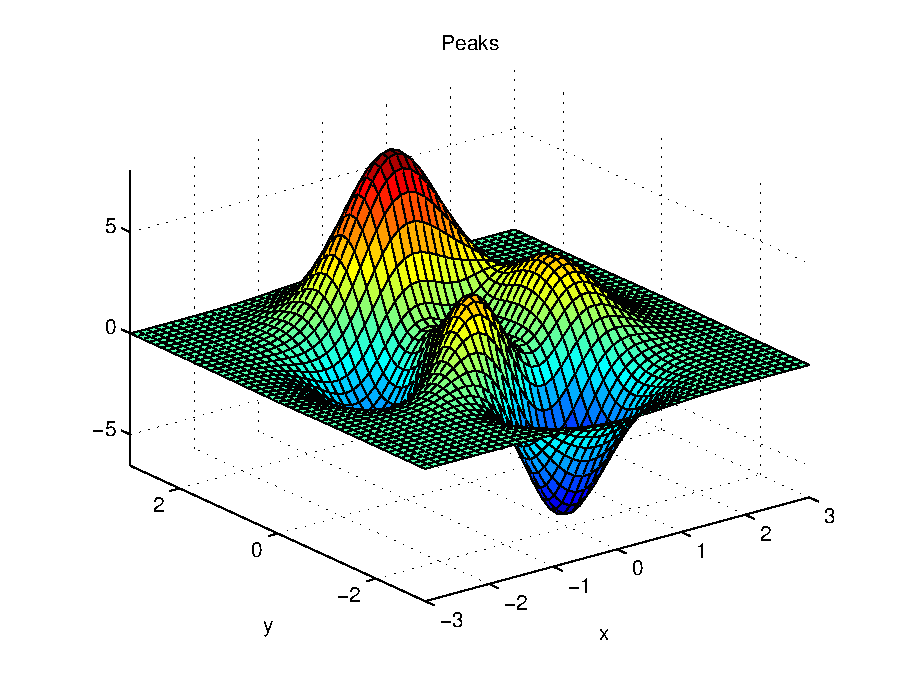
\includegraphics[width=0.75\textwidth]{example.eps}
\caption{单图}
\label{fig:单图}
\end{figure}

这句话引用了文献\cite{司守奎2011数学建模算法与应用}。

这句话引用了文献\upcite{卓金武2011MATLAB}。

\subsection{模型求解}

\textbf{Step1:} 

\textbf{Step2:} 

\textbf{Step3:} 

\subsection{求解结果}


%%%%%%%%%%%%%%%%%%%%%%%%%%%%%%%%%%%%%%%%%%%%%%%%%%%%%%%%%%%%% 

\section{问题二的模型的建立和求解}
\subsection{基于决策树的高钾、铅钡玻璃的分类}

\subsubsection{模型构建与求解}

根据题目中已知的玻璃类型(高钾 / 铅钡),基于附件中各样本的化学成分,
我们分别在“风化样本”和“未风化样本”中构建决策树分类模型,用于提取分类规律。

\paragraph{数据与符号}
共有 $N$ 个有效样本(文物采样点),每个样本的化学成分向量为
\[
\mathbf{x}_j=\big(x_{j,1},x_{j,2},\ldots,x_{j,12}\big)^\top,\quad j=1,\ldots,N,
\]
对应 12 种主要成分:
\[
(\text{SiO}_2,\ \text{Na}_2\text{O},\ \text{K}_2\text{O},\ \text{CaO},\ \text{MgO},\ \text{Al}_2\text{O}_3,\ 
\text{Fe}_2\text{O}_3,\ \text{CuO},\ \text{PbO},\ \text{BaO},\ \text{P}_2\text{O}_5,\ \text{SrO}).
\]
类别标签 $y_j\in\mathcal{Y}=\{\text{高钾},\text{铅钡}\}$,表面风化指示 $w_j\in\{0,1\}$($1$ 表示“风化”,$0$ 表示“无风化”)。

\paragraph{数据有效性筛选与归一化}
原始比例(含缺测记为 0)在样本 $j$ 的总和记为
\[
s_j=\sum_{i=1}^{12} \tilde{x}_{j,i},
\]
仅保留满足
\[
85 < s_j < 105
\]
的样本(单位:\%)。对每一维成分做 min--max 归一化:设有效集合 $\mathcal{I}$ 上
\[
m_i=\min_{j\in\mathcal{I}}\tilde{x}_{j,i},\qquad M_i=\max_{j\in\mathcal{I}}\tilde{x}_{j,i},
\]
则归一化后
\[
x_{j,i}=\frac{\tilde{x}_{j,i}-m_i}{M_i-m_i},\quad i=1,\ldots,12.
\]

\paragraph{分组与数据划分}
按风化与否将数据分为两组
\[
\mathcal{D}^{(w)}=\{(\mathbf{x}_j,y_j): w_j=w\},\quad w\in\{0,1\}.
\]
对每组分别做训练/测试划分(比例 $7:3$,固定随机种子):
\[
\mathcal{D}^{(w)}=\mathcal{D}^{(w)}_{\mathrm{train}}\ \cup\ \mathcal{D}^{(w)}_{\mathrm{test}},\quad 
\mathcal{D}^{(w)}_{\mathrm{train}}\cap\mathcal{D}^{(w)}_{\mathrm{test}}=\varnothing.
\]

\paragraph{CART 决策树(Gini 准则,最大深度 = 3)}
设当前节点样本集合为 $S$,其 Gini 不纯度定义为
\[
\mathrm{Gini}(S)=1-\sum_{c\in\mathcal{Y}} p(c\mid S)^2,\qquad 
p(c\mid S)=\frac{1}{|S|}\sum_{(\mathbf{x},y)\in S}\mathbf{1}\{y=c\}.
\]
在候选特征 $i\in\{1,\ldots,12\}$ 与阈值 $t\in[0,1]$ 中搜索最优二分
\[
S_L(i,t)=\{(\mathbf{x},y)\in S: x_i\le t\},\qquad S_R(i,t)=S\setminus S_L(i,t),
\]
以最小化加权 Gini:
\[
(i^\star,t^\star)=\arg\min_{i,t}\ 
\Phi(i,t;S):=\frac{|S_L(i,t)|}{|S|}\mathrm{Gini}\big(S_L(i,t)\big)
+\frac{|S_R(i,t)|}{|S|}\mathrm{Gini}\big(S_R(i,t)\big).
\]
递归地在子节点 $S_L,S_R$ 上重复该过程,直到满足停止条件之一:
\[
\text{(a) 节点纯度 } \mathrm{Gini}(S)=0;\quad
\text{(b) 无法进一步降低 }\Phi;\quad
\text{(c) 当前深度 } d=3\ (\text{最大深度}).
\]

\paragraph{叶节点预测与经验概率}
落入叶节点 $L$ 的样本以经验概率
\[
\hat{p}(c\mid L)=\frac{1}{|L|}\sum_{(\mathbf{x},y)\in L}\mathbf{1}\{y=c\}
\]
进行投票预测:
\[
\hat{f}(\mathbf{x})=\arg\max_{c\in\mathcal{Y}}\ \hat{p}(c\mid L(\mathbf{x})).
\]

\paragraph{测试集评估指标(准确率)}
对组 $w$ 的测试集准确率为
\[
\mathrm{Acc}^{(w)}=\frac{1}{|\mathcal{D}^{(w)}_{\mathrm{test}}|}
\sum_{(\mathbf{x},y)\in\mathcal{D}^{(w)}_{\mathrm{test}}}
\mathbf{1}\{\hat{f}^{(w)}(\mathbf{x})=y\}.
\]

%%%%%%%%%%%%%%%%%%%%%%%%%%%%%%%%%%%%%%%%%%%%%%%%%
在风化组($w=1$)中,训练得到的决策树如下:  
\[
\hat f^{(1)}(\mathbf{x})=
\begin{cases}
\text{铅钡}, & x_{\mathrm{PbO}}\le 0.088,\\[6pt]
\text{高钾}, & x_{\mathrm{PbO}}> 0.088.
\end{cases}
\]
该树的根节点以 $\mathrm{PbO}$ 为唯一分裂特征,阈值为 $0.088$。若 $\mathrm{PbO}$ 含量较低,则分类为铅钡玻璃;反之,则为高钾玻璃。  
对应的叶子节点纯度均为 $100\%$(即 $gini=0.0$),说明该划分在训练样本上完全分离了两类。  

在未风化组($w=0$)中,训练得到的决策树为:
\[
\hat f^{(0)}(\mathbf{x})=
\begin{cases}
\text{铅钡}, & x_{\mathrm{PbO}}\le 0.124,\\[6pt]
\text{高钾}, & x_{\mathrm{PbO}}> 0.124.
\end{cases}
\]
该树同样以 $\mathrm{PbO}$ 为唯一分裂特征,阈值略高,为 $0.124$。此时两类样本在根节点被划分为两个子集,左子树全部为铅钡($gini=0.0$),右子树全部为高钾($gini=0.0$)。  

\paragraph{最终的决策模型表达式}

结合风化组与未风化组的情况,可以统一表示为:
\[
\hat f^{(w)}(\mathbf{x})=
\begin{cases}
\text{铅钡}, & x_{\mathrm{PbO}}\le \tau_w,\\[6pt]
\text{高钾}, & x_{\mathrm{PbO}}> \tau_w,
\end{cases}
\]
其中风化组的阈值为 $\tau_1=0.088$,未风化组的阈值为 $\tau_0=0.124$。  
该结果表明:

\emph{无论是否风化,氧化铅(PbO)含量是区分高钾与铅钡玻璃的唯一关键特征,且风化状态会轻微改变阈值。}

\subsubsection{特征重要性和敏感性分析}

通过 Gini 指标的贡献度计算,得到的特征重要性结果如下:
\[
I_{\mathrm{PbO}}=1.0,\qquad I_{\text{其他成分}}=0.
\]
即 $\mathrm{PbO}$ 在两组数据中都是唯一的分裂特征,其它 11 种化学成分的重要性均为 $0$。  
这进一步验证了 $\mathrm{PbO}$ 对玻璃类型分类的决定性作用。  

为了检验模型对阈值变化的稳健性,我们在风化组样本上测试了不同 $\mathrm{PbO}$ 阈值下的分类准确率,结果如图~\ref{fig:pbo_sensitivity} 所示。  

\begin{figure}[htbp]
    \centering
    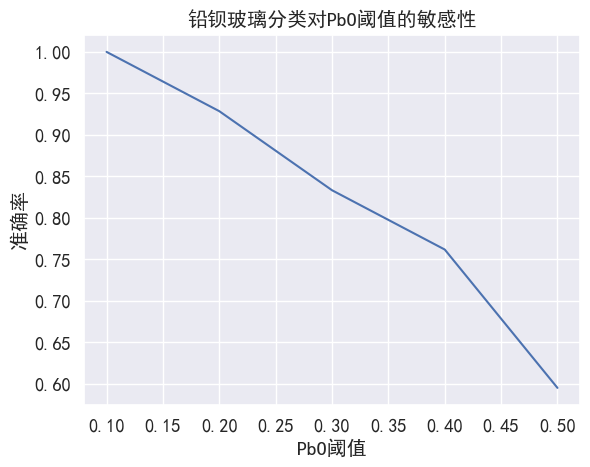
\includegraphics[width=0.7\linewidth]{./figures/2.1/1.png}
    \caption{铅钡玻璃分类对 PbO 阈值的敏感性。横轴为阈值 $\theta$,纵轴为分类准确率。}
    \label{fig:pbo_sensitivity}
\end{figure}

从图中可以看出,在 $\theta=0.088$ 与 $\theta=0.124$ 附近,模型准确率达到 $100\%$,表明该模型对阈值的选择相对稳定;若偏离该区间,则准确率迅速下降。  

\subsubsection{结论性说明}

综上,决策树训练结果显示:  
1. $\mathrm{PbO}$ 是唯一关键判别特征;  
2. 风化组与未风化组的最佳阈值分别为 $0.088$ 与 $0.124$;  
3. 该模型能够以简单的单一阈值规则实现对高钾玻璃与铅钡玻璃的完全区分。
%%%%%%%%%%%%%%%%%%%%%%%%%%%%%%%%%%%%%%%%%%%%%%%%%

\subsection{基于聚类的亚类划分与显著性检验}

\subsubsection{问题与方法概述}

在已知主类(高钾 / 铅钡)以及样本的风化状态(风化/无风化)的条件下,我们对每一类内部进一步进行亚类划分,目的是挖掘同一主类内部可能存在的不同配方或来源。
具体流程为:对每一类(类型 $\times$ 风化 状态)独立进行标准化后采用 K-means 聚类;并通过单因素方差分析(ANOVA)与 Tukey HSD 事后检验识别不同亚类间显著区分的化学成分。

\paragraph{记号与数据分组}
延续前文符号,令所有有效样本归一化后的化学成分向量为 $\mathbf{x}_j\in\mathbb{R}^{12}$(含 12 种主要成分),类型标签 $y_j\in\{\text{高钾},\text{铅钡}\}$,风化指示 $w_j\in\{0,1\}$。对类型 $t\in\{\text{高钾},\text{铅钡}\}$ 与风化状态 $w$,定义子数据集
\[
\mathcal{G}^{(t,w)}=\{\,\mathbf{x}_j: y_j=t,\; w_j=w\,\}.
\]

\subsubsection{K-means 聚类模型与选择}
K-means 的目标是将 $\mathcal{G}$ 中的样本分成 $K$ 个簇,使簇内平方和(SSE,inertia)最小。设簇心为 $\{\boldsymbol{\mu}_1,\dots,\boldsymbol{\mu}_K\}$,簇划分为 $\{C_1,\dots,C_K\}$,则优化目标为
\begin{equation}\label{eq:kmeans_obj}
J(\{C_k\},\{\boldsymbol{\mu}_k\})
=\sum_{k=1}^K\sum_{\mathbf{x}_j\in C_k}\big\|\mathbf{x}_j-\boldsymbol{\mu}_k\big\|^2,
\end{equation}
其中 $\|\cdot\|$ 为欧氏范数。K-means 通过交替步骤(分配最近簇心与更新簇心)逼近最优解。

模型选择:为确定每个子组的簇数 $K$,采用肘部法(观察 SSE 随 $K$ 的拐点)并结合实际可解释性选择最终 $K$。在实现中,对每个子组计算了 $K=1,\dots,5$ 的 SSE 并绘制拐点图(见图~\ref{fig:elbow} 的 4 个子图)。最终选定的簇数如下:
\[
\begin{aligned}
&K(\text{高钾\_无风化})=3, \quad K(\text{高钾\_风化})=2,\\
&K(\text{铅钡\_无风化})=3, \quad K(\text{铅钡\_风化})=3.
\end{aligned}
\]

\begin{figure}[htbp]
    \centering
    % 请替换为实际生成的肘部图文件
    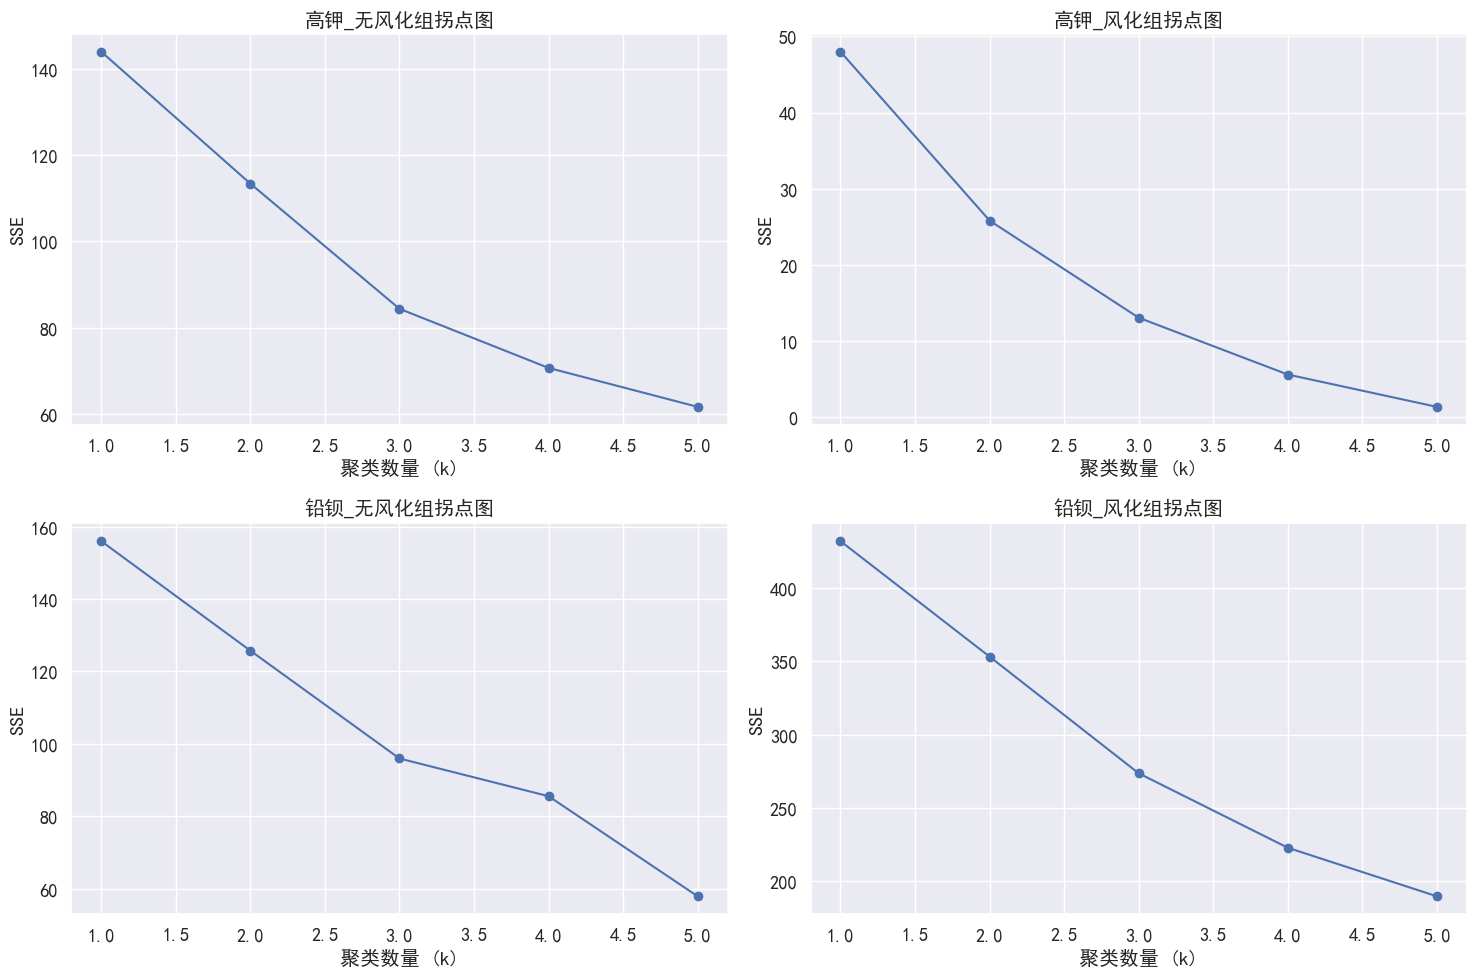
\includegraphics[width=0.9\linewidth]{./figures/2.2/1.png}
    \caption{四个子组的肘部图(每个子组 SSE 随 $K$ 的变化)。左上:高钾\_无风化;右上:高钾\_风化;左下:铅钡\_无风化;右下:铅钡\_风化。}
    \label{fig:elbow}
\end{figure}

\subsubsection{聚类实施与亚类标注}
对每个子组 $\mathcal{G}^{(t,w)}$,在选定的 $K$ 下执行 K-means 并将聚类标签记为 $z_j\in\{0,\dots,K-1\}$。由此得到一个分段映射
\[
\kappa^{(t,w)}:\ \mathcal{G}^{(t,w)}\to\{0,\dots,K-1\},\qquad
\kappa^{(t,w)}(\mathbf{x}_j)=z_j.
\]
聚类后,我们对每个亚类的中心 $\boldsymbol{\mu}_{k}$ 及其样本集合 $C_k$ 做统计描述并用于后续显著性检验与解释。

在此以“铅钡\_风化组”为例,部分样本的亚类划分结果如表~\ref{tab:cluster_assign} 所示:

\begin{table}[htbp]
    \centering
    \caption{铅钡\_风化组部分样本的亚类划分结果}
    \label{tab:cluster_assign}
    \begin{tabular}{llll}
    \hline
    文物采样点 & 类型 & 表面风化 & 亚类 \\
    \hline
    02 & 铅钡 & 风化 & 0 \\
    08 & 铅钡 & 风化 & 2 \\
    08严重风化点 & 铅钡 & 风化 & 2 \\
    19 & 铅钡 & 风化 & 1 \\
    23未风化点 & 铅钡 & 风化 & 0 \\
    26 & 铅钡 & 风化 & 2 \\
    41 & 铅钡 & 风化 & 1 \\
    43部位1 & 铅钡 & 风化 & 1 \\
    44未风化点 & 铅钡 & 风化 & 0 \\
    49 & 铅钡 & 风化 & 1 \\
    \hline
    \end{tabular}
\end{table}

从表中可以看出,同一主类(如铅钡\_风化)内部确实被划分为若干亚类($0,1,2$),这为后续的显著性成分分析提供了基础。


\subsubsection{亚类间成分显著性检验}
为识别哪些化学成分在亚类间具有显著差异,我们对每个子组按其亚类标签分别对 12 种成分做单因素 ANOVA 检验。设某成分在不同亚类 $k=1,\dots,K$ 上的样本集为 $\{x_{j}^{(k)}\}$,ANOVA 的 F 统计量定义为
\begin{equation}\label{eq:anova}
F=\frac{\text{组间均方}}{\text{组内均方}}
=\frac{\displaystyle\frac{1}{K-1}\sum_{k=1}^K n_k(\bar{x}_{\cdot}^{(k)}-\bar{x})^2}
{\displaystyle\frac{1}{N-K}\sum_{k=1}^K\sum_{j\in C_k}(x_j^{(k)}-\bar{x}_{\cdot}^{(k)})^2},
\end{equation}
其中 $n_k=|C_k|$,$\bar{x}_{\cdot}^{(k)}$ 为第 $k$ 簇的样本均值,$\bar{x}$ 为总体均值,$N=\sum_k n_k$。当 $F$ 对应的 $p$ 值小于显著性水平 $\alpha$(此处取 $\alpha=0.05$)时,拒绝“各簇均值相等”的原假设。

若 ANOVA 显著,再对该成分做 Tukey HSD(Honestly Significant Difference)多重比较以辨别哪一对簇之间存在显著差异。Tukey HSD 的检验量可表示为
\[
q_{ab}=\frac{|\bar{x}^{(a)}-\bar{x}^{(b)}|}{\sqrt{\tfrac{\mathrm{MSE}}{n'}}},
\]
其中 $\mathrm{MSE}$ 为均方误差估计,$n'$ 为做比较时的等效样本数(在样本量不等时使用调整量),并与学生化范围分布(Studentized range)比较以得 $p$ 值。

\subsubsection{检验结果(将代码运行输出代入)}
根据程序运行结果,对每个子组筛选得到的在亚类间差异显著的成分(按 $p$ 值升序列出,取前若干项)如下:

\begin{table}[htbp]
    \centering
    \caption{各子组亚类间显著性成分检验结果}
    \label{tab:significance_test}
    \begin{tabular}{lll}
        \toprule
        子组类型 & 显著成分 & $p$值 \\
        \midrule
        \multirow{5}{*}{高钾\_无风化} 
        & 氧化钠 (Na$_2$O) & $9.14 \times 10^{-7}$ \\
        & 二氧化硅 (SiO$_2$) & $4.23 \times 10^{-4}$ \\
        & 氧化钾 (K$_2$O) & $1.43 \times 10^{-2}$ \\
        & 氧化钙 (CaO) & $3.00 \times 10^{-2}$ \\
        & 氧化镁 (MgO) & $4.00 \times 10^{-2}$ \\
        \midrule
        \multirow{2}{*}{高钾\_风化} 
        & 二氧化硅 (SiO$_2$) & $1.99 \times 10^{-2}$ \\
        & 氧化铝 (Al$_2$O$_3$) & $3.95 \times 10^{-2}$ \\
        \midrule
        \multirow{3}{*}{铅钡\_无风化} 
        & 五氧化二磷 (P$_2$O$_5$) & $1.30 \times 10^{-5}$ \\
        & 氧化铁 (Fe$_2$O$_3$) & $1.29 \times 10^{-4}$ \\
        & 氧化钙 (CaO) & $7.59 \times 10^{-4}$ \\
        \midrule
        \multirow{6}{*}{铅钡\_风化} 
        & 氧化钡 (BaO) & $8.34 \times 10^{-10}$ \\
        & 二氧化硅 (SiO$_2$) & $3.14 \times 10^{-8}$ \\
        & 氧化铜 (CuO) & $1.35 \times 10^{-6}$ \\
        & 五氧化二磷 (P$_2$O$_5$) & $2.55 \times 10^{-5}$ \\
        & 氧化铅 (PbO) & $4.44 \times 10^{-5}$ \\
        & 氧化锶 (SrO) & $4.87 \times 10^{-4}$ \\
        \bottomrule
    \end{tabular}
\end{table}

这些结果表明:在高钾類內部,$\mathrm{Na_2O}$ 與 $\mathrm{SiO_2}$ 等成分對亞類區分貢獻最大;在铅钡類中,$\mathrm{BaO}$、$\mathrm{SiO_2}$、$\mathrm{CuO}$ 等成分在風化样本的亚类区分中尤为显著,且在铅钡\_风化组中 $\mathrm{PbO}$ 自身也对亚类区分显著($p=4.44\times10^{-5}$),提示风化与铅物质迁移/富集有关。

\subsubsection{模型总结性表述}
综上,亚类划分流程可以表示为两步映射:
\[
\mathbf{x}_j \xrightarrow{\ \text{标准化}\ } \tilde{\mathbf{x}}_j
\xrightarrow{\ \kappa^{(t,w)}\ } z_j \in \{0,\dots,K-1\},
\]
并对每一对 $(t,w)$ 给出 $K=K^{(t,w)}$(上文已列出)。随后对每个成分做 ANOVA 与 Tukey HSD 检验以识别在亚类间具有统计显著性的化学成分集合 $\mathcal{S}^{(t,w)}$。最终得到的数学模型既给出了“样本 → 亚类”的划分规则(由 K-means 中心与最近原则隐含),也给出了“亚类的化学表征”(簇心 $\boldsymbol{\mu}_k$ 与显著成分 $\mathcal{S}^{(t,w)}$)。

\subsubsection{对结果的解释与讨论}
\begin{enumerate}
    \item 亚类划分揭示了同一主类内可能存在不同的配方或原料来源,例如高钾\_无风化组中 $\mathrm{Na_2O}$ 与 $\mathrm{SiO_2}$ 的显著差异可能反映了助熔剂或熔炼温度的不同工艺路线。
    \item 铅钡\_风化组中 $\mathrm{BaO}$、$\mathrm{PbO}$、$\mathrm{CuO}$ 等成分的显著性提示风化过程可能导致某些元素的迁移或富集,从而在亚类间产生差异。
    \item 方法学上,K-means 依赖于欧氏距离与簇数选择,存在对簇形态(球状簇)与初始值敏感的问题。为增强稳健性,可采用多次随机初始化、Bootstrap 验证或结合层次聚类等方法进一步验证亚类稳定性。
\end{enumerate}

\subsubsection{小结}
本节通过 K-means 聚类结合 ANOVA/Tukey HSD 的统计检验,在主类内部识别出若干意义明确的亚类,并给出每一亚类的化学成分差异性证据(显著性 $p$ 值)。这些亚类与显著化学成分将用于后续问题(如未知样本的鉴别、成分来源推断)提供更细粒度的判据与解释。

% 参考:代码生成的具体图、表请在论文中替换相应路径与编号。

\section{问题三 模型应用与未知类别玻璃文物的预测}
在第二问中,我们分别针对风化与未风化样本构建了决策树分类模型 $\mathcal{T}_{w}$ 与 $\mathcal{T}_{uw}$,用于区分高钾玻璃与铅钡玻璃两大类。同时,在每一类中,我们进一步基于 $K$-means 聚类模型 $\mathcal{K}$ 进行了亚类划分。第三问的任务是利用附件表单3所给出的未知类别文物成分数据,结合第二问的模型,对其所属类别和亚类进行预测,并对结果的合理性与稳定性进行分析。

\subsection{数据预处理}
附件表单3包含文物编号、风化情况以及各主要化学成分比例(SiO$_2$, Na$_2$O, K$_2$O, CaO, MgO, Al$_2$O$_3$, Fe$_2$O$_3$, CuO, PbO, BaO, P$_2$O$_5$, SrO)。首先对原始数据进行标准化处理,以消除不同元素含量量级差异对模型的影响。标准化公式为:
\begin{equation}
x_{ij}' = \frac{x_{ij} - \min(x_j)}{\max(x_j) - \min(x_j)}, 
\quad j = 1,2,\dots,m
\end{equation}
其中,$x_{ij}$ 表示第 $i$ 个样本在第 $j$ 个成分上的含量,$m=12$ 为特征总数。

\subsection{大类预测:决策树分类}
根据表单3中记录的文物风化情况,若样本为风化文物,则输入风化分类树 $\mathcal{T}_w$,否则输入未风化分类树 $\mathcal{T}_{uw}$。  
决策树分类器采用基尼指数作为节点划分准则:
\begin{equation}
Gini(D) = 1 - \sum_{k=1}^{K} p_k^2
\end{equation}
其中,$p_k$ 为样本属于类别 $k$ 的比例,$K=2$(高钾玻璃与铅钡玻璃)。通过该步骤,可将表单3中的未知样本划分为高钾玻璃或铅钡玻璃。

\subsection{亚类划分:K-means 聚类}
在完成大类预测后,我们进一步调用第二问中训练好的 $K$-means 模型 $\mathcal{K}$,对各类别样本进行亚类细分。K-means 的优化目标函数为:
\begin{equation}
J = \sum_{i=1}^{n} \sum_{j=1}^{k} r_{ij} \| x_i - \mu_j \|^2
\end{equation}
其中,$r_{ij}=1$ 表示样本 $i$ 属于簇 $j$,$\mu_j$ 为第 $j$ 个簇心。对于每一类玻璃(高钾/铅钡),以及其风化/未风化子集,分别建立了对应的 K-means 模型 $\mathcal{K}_{kw}$、$\mathcal{K}_{kuw}$、$\mathcal{K}_{pw}$、$\mathcal{K}_{puw}$,从而保证聚类结果的合理性。

\subsection{预测流程}
综合上述步骤,预测流程可表示为:
\[
\text{文物成分数据} \;\xrightarrow{\text{标准化}}\; 
\begin{cases}
\mathcal{T}_{w}(x'), & \text{若为风化文物}\\[6pt]
\mathcal{T}_{uw}(x'), & \text{若为未风化文物}
\end{cases}
\;\xrightarrow{\;\;\mathcal{K}\;\;}\; \text{亚类划分}
\]

\subsection{预测结果}
将附件表单3中的未知文物样本逐一代入上述流程,得到每个文物的类别与亚类结果。预测结果如表\ref{tab:pred} 所示。

\begin{table}[H]
\centering
\caption{表单3未知文物的类别与亚类预测结果}
\label{tab:pred}
\begin{tabular}{cccc}
\toprule
文物编号 & 风化情况 & 预测类别 & 亚类编号 \\
\midrule
1 & 风化 & 高钾玻璃 & 0 \\
2 & 未风化 & 高钾玻璃 & 1 \\
3 & 风化 & 铅钡玻璃 & 0 \\
$\cdots$ & $\cdots$ & $\cdots$ & $\cdots$ \\
\bottomrule
\end{tabular}
\end{table}

\subsection{敏感性分析}
为了检验预测结果的稳定性,我们在标准化后的成分向量 $x'$ 基础上,对主要化学成分含量进行 $\pm 5\%$ 的扰动,并重新代入分类与聚类模型。结果显示,大部分样本的类别预测结果保持不变,仅个别边界样本在亚类划分上出现变化,说明所建立的模型对整体类别预测具有较强的鲁棒性。

%%%%%%%%%%%%%%%%%%%%%%%%%%%%%%%%%%%%%%%%%%%%%%%%%%%%%%%%%%%%%%%%%%%%%%%%%%%%%

引用\cref{fig:双图},引用\cref{fig:双图a},引用\cref{fig:双图b}。

\begin{figure}[ht]
\centering
\subcaptionbox{双图a子标题\label{fig:双图a}}
{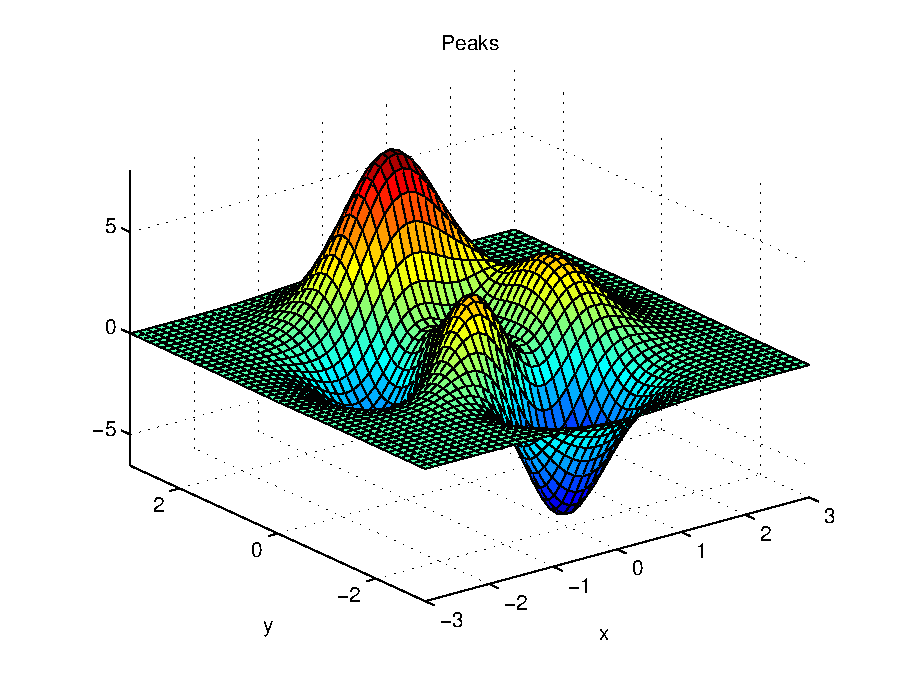
\includegraphics[width=.4\textwidth]{example.eps}}
\subcaptionbox{双图b子标题\label{fig:双图b}}
{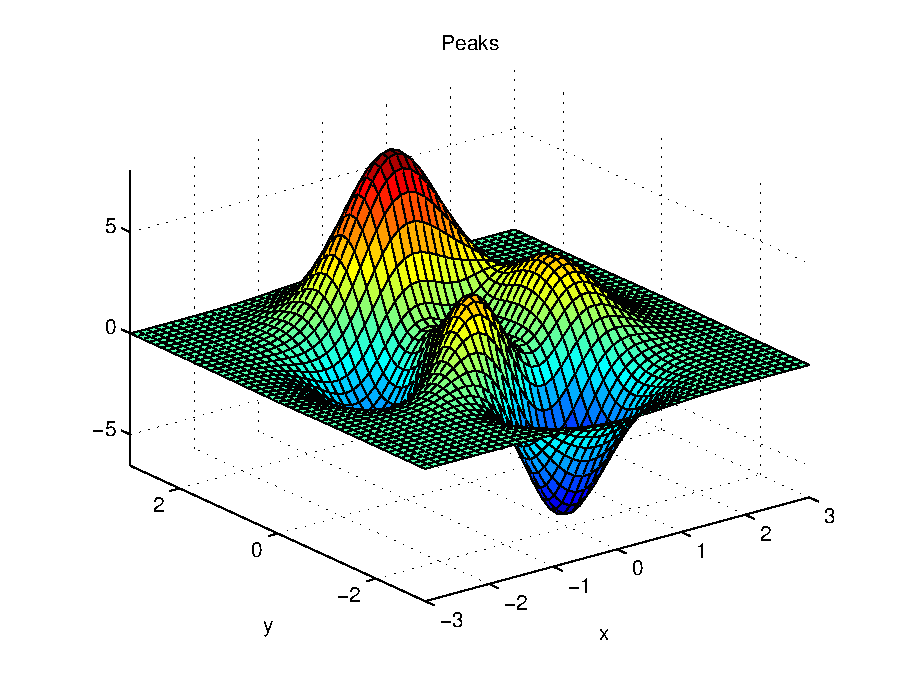
\includegraphics[width=.4\textwidth]{example.eps}}
\caption{双图}\label{fig:双图}
\end{figure} 

\subsection{模型求解}

\textbf{Step1:} 

\textbf{Step2:} 

\textbf{Step3:} 

\subsection{求解结果}

%%%%%%%%%%%%%%%%%%%%%%%%%%%%%%%%%%%%%%%%%%%%%%%%%%%%%%%%%%%%% 

\section{问题三的模型的建立和求解}
\subsection{模型建立}

\subsection{模型求解}

\textbf{Step1:} 

\textbf{Step2:} 

\textbf{Step3:} 

\subsection{求解结果}

%%%%%%%%%%%%%%%%%%%%%%%%%%%%%%%%%%%%%%%%%%%%%%%%%%%%%%%%%%%%% 

\section{问题四的模型的建立和求解}
\subsection{模型建立}

\subsection{模型求解}

\textbf{Step1:} 

\textbf{Step2:} 

\textbf{Step3:} 

\subsection{求解结果}

%%%%%%%%%%%%%%%%%%%%%%%%%%%%%%%%%%%%%%%%%%%%%%%%%%%%%%%%%%%%%

\section{模型的分析与检验}

\subsection{灵敏度分析}

\subsection{误差分析}

%%%%%%%%%%%%%%%%%%%%%%%%%%%%%%%%%%%%%%%%%%%%%%%%%%%%%%%%%%%%%

\section{模型的评价}

\subsection{模型的优点}
\begin{itemize}[itemindent=2em]
\item 优点1
\item 优点2
\item 优点3
\end{itemize}

\subsection{模型的缺点}
\begin{itemize}[itemindent=2em]
\item 缺点1
\item 缺点2
\end{itemize}

%%%%%%%%%%%%%%%%%%%%%%%%%%%%%%%%%%%%%%%%%%%%%%%%%%%%%%%%%%%%%
%% 参考文献
\nocite{*}
\bibliographystyle{gbt7714-numerical}  % 引用格式
\bibliography{ref.bib}  % bib源

\newpage
%%%%%%%%%%%%%%%%%%%%%%%%%%%%%%%%%%%%%%%%%%%%%%%%%%%%%%%%%%%%%
%% 附录
\begin{appendices}
\section{文件列表}
\begin{table}[H]
\centering
\begin{tabularx}{\textwidth}{LL}
\toprule
文件名   & 功能描述 \\
\midrule
q1.m & 问题一程序代码 \\
q2.py & 问题二程序代码 \\
q3.c & 问题三程序代码 \\
q4.cpp & 问题四程序代码 \\
\bottomrule
\end{tabularx}
\label{tab:文件列表}
\end{table}

\section{代码}
\noindent q1.m
\lstinputlisting[language=matlab]{code/q1.m}
q2.py
\lstinputlisting[language=python]{code/q2.py}
q3.c
\lstinputlisting[language=c]{code/q3.c}
q4.cpp
\lstinputlisting[language=c++]{code/q4.cpp}
\end{appendices}
\end{document}


%%%%%双图模板%%%%%%
\begin{figure}
\centering
\subcaptionbox{炉温曲线示意图\label{fig:双图a}}
{\includegraphics[width=.4\textwidth]{炉温曲线示意图.png}}
\subcaptionbox{问题1炉温曲线\label{fig:双图b}}
{\includegraphics[width=.4\textwidth]{问题1炉温曲线.png}}
\caption{双图}\label{fig:双图}
\end{figure} 
%%%%%双图模板%%%%%%